\documentclass[11pt,a4paper]{article}

%%%%%%%%%%%%%%%%%%%%%%%%%%%%%%%%%%%%%%%%%%%%%%%%%%%%%%%%%%%%%%%%%%%%%%%%
%%  Efficient Deep Learning Systems -- Lecture 9: Inference           %%
%%  Acceleration and Compression of Large Language Models             %%
%%  Lecture notes, cleaned and typeset (design matches Lecture 1).    %%
%%  Links from the lecture slides added as footnotes / \href.         %%
%%%%%%%%%%%%%%%%%%%%%%%%%%%%%%%%%%%%%%%%%%%%%%%%%%%%%%%%%%%%%%%%%%%%%%%%

% ---- Packages ----
\usepackage[utf8]{inputenc}
\usepackage[T1]{fontenc}
\usepackage[english]{babel}

\usepackage[margin=1.1in]{geometry}
\usepackage{amsmath, amssymb, amsthm, mathtools}
\usepackage{booktabs, array}
\usepackage{enumitem}
\usepackage{xcolor}
\usepackage{graphicx}
\usepackage{epigraph}
\usepackage{csquotes}
\usepackage{tikz}
\usetikzlibrary{arrows.meta, positioning, shapes.geometric, shapes.misc,
                fit, calc, backgrounds, decorations.pathreplacing,
                patterns, matrix}
\usepackage{pgfplots}
\pgfplotsset{compat=1.18}

\usepackage[colorlinks=true, linkcolor=black!70!blue,
            citecolor=black!70!blue, urlcolor=black!40!blue]{hyperref}

% ---- Theorem environments ----
\theoremstyle{definition}
\newtheorem{definition}{Definition}[section]
\newtheorem{example}[definition]{Example}

\theoremstyle{remark}
\newtheorem*{remark}{Remark}
\newtheorem*{aside}{Aside}
\newtheorem*{principle}{Design principle}

\theoremstyle{plain}
\newtheorem{proposition}[definition]{Proposition}
\newtheorem{theorem}[definition]{Theorem}

% ---- Epigraph style ----
\setlength{\epigraphwidth}{0.6\textwidth}
\renewcommand{\epigraphflush}{flushright}
\renewcommand{\textflush}{flushright}
\renewcommand{\epigraphsize}{\small\itshape}

% ---- Small conveniences ----
\newcommand{\todo}[1]{\textcolor{red!70!black}{\textbf{[TODO: #1]}}}
\DeclareMathOperator*{\argmin}{arg\,min}
\newcommand{\R}{\mathbb{R}}
\newcommand{\E}{\mathbb{E}}
\newcommand{\softmax}{\operatorname{softmax}}
\newcommand{\clip}{\operatorname{clip}}
\newcommand{\KL}{D_{\mathrm{KL}}}
\newcommand{\bigO}{\mathcal{O}}
\newcommand{\arxivlink}[1]{\href{https://arxiv.org/abs/#1}{arXiv:#1}}

% ---- Diagram palette ----
\definecolor{accent}{RGB}{30,70,130}
\definecolor{defgreen}{RGB}{35,110,60}
\definecolor{remarkorange}{RGB}{180,90,20}

% ---- Title ----
\title{\textbf{Efficient Deep Learning Systems} \\[0.3em]
       \large Lecture 9 --- Inference Acceleration and Compression \\
       of Large Language Models}
\author{Lecture notes \\[0.2em]
        \small Guest lecture by Roman Gorb, YandexGPT Inference Acceleration Team}
\date{}

\begin{document}
\sloppy
\maketitle

\begin{abstract}
\noindent
These notes give a self-contained, reference-linked account of inference
acceleration and compression for large language models. We begin with the
GPU memory/compute hierarchy and the resulting \emph{compute-bound} /
\emph{memory-bound} dichotomy, formalise the \emph{prefill}/\emph{decoding}
split, and then proceed through quantization (GPTQ, SmoothQuant, FP8, the
rotation-based SpinQuant family, and the block formats MXFP4/NVFP4),
architectural responses (grouped-query attention, Mixture-of-Experts),
KV-cache management and sparse attention, speculative decoding
(rejection-sampling theory, EAGLE/EAGLE-2/EAGLE-3), linear-attention /
state-space hybrids, and knowledge distillation. Each technique is given
its governing equations, its quantitative trade-offs, and a citation to
the primary source; a consolidated reference list appears in
Section~\ref{sec:refs}. The organising claim is that no optimisation is
free: every speedup is purchased by spending some other resource---precision,
memory, training compute, or architectural generality---and the central
skill of an inference engineer is identifying which resource is locally
cheapest.
\end{abstract}

\tableofcontents
\bigskip
\hrule
\bigskip

%%%%%%%%%%%%%%%%%%%%%%%%%%%%%%%%%%%%%%%%%%%%%%%%%%%%%%%%%%%%%%%%%%%%%%%%
\section{Introduction: The Compression Imperative}
%%%%%%%%%%%%%%%%%%%%%%%%%%%%%%%%%%%%%%%%%%%%%%%%%%%%%%%%%%%%%%%%%%%%%%%%

Deploying a large language model in production is an exercise in
disciplined compromise. A model that attains state-of-the-art accuracy on
academic benchmarks but requires ten seconds to emit a single token is, in
the commercial sense, no model at all. The entire discipline of
\emph{inference acceleration} is thus devoted to the question: given a
fixed computational budget, how may we preserve as much of a model's
capability as possible while reducing its resource footprint?

These notes trace the standard arc of this discipline. We begin with the
hardware substrate---the GPU and its memory hierarchy---because every
subsequent technique is ultimately a response to the constraints it
imposes. We then examine the two operational phases of transformer
inference, \emph{context processing} and \emph{decoding}, and show that
they exhibit fundamentally different computational profiles. From there
we survey the principal families of compression techniques---quantization,
architectural surgery, cache management, speculative decoding, and
knowledge distillation---each responding to a particular aspect of the
cost equation.

%%%%%%%%%%%%%%%%%%%%%%%%%%%%%%%%%%%%%%%%%%%%%%%%%%%%%%%%%%%%%%%%%%%%%%%%
\section{The Hardware Substrate: GPU Memory and Compute}
\label{sec:hardware}
%%%%%%%%%%%%%%%%%%%%%%%%%%%%%%%%%%%%%%%%%%%%%%%%%%%%%%%%%%%%%%%%%%%%%%%%

Before we can speak meaningfully of acceleration, we must speak of the
machine. A modern GPU is not simply ``a fast chip''; it is a carefully
stratified hierarchy in which the speed of arithmetic is matched against
the far slower speed of data movement. The overwhelming majority of
optimisations discussed in these notes are, at their core, attempts to
keep the arithmetic units fed. The slides point to an article on Habr
(Yandex's engineering blog) for background on GPU architecture and its
limitations.\footnote{\url{https://habr.com/en/companies/yandex/articles/672396/}}

\subsection{Cores and the Memory Hierarchy}

A contemporary GPU exposes two principal classes of compute unit: the
general-purpose \textbf{CUDA cores}, inherited from the graphics lineage,
and the specialised \textbf{Tensor cores}, which perform small matrix
multiplications at extraordinarily high throughput and are the workhorses
of deep learning.

Surrounding these compute units is a three-tier memory hierarchy, each
tier exhibiting a characteristic trade-off between capacity and latency:

\begin{center}
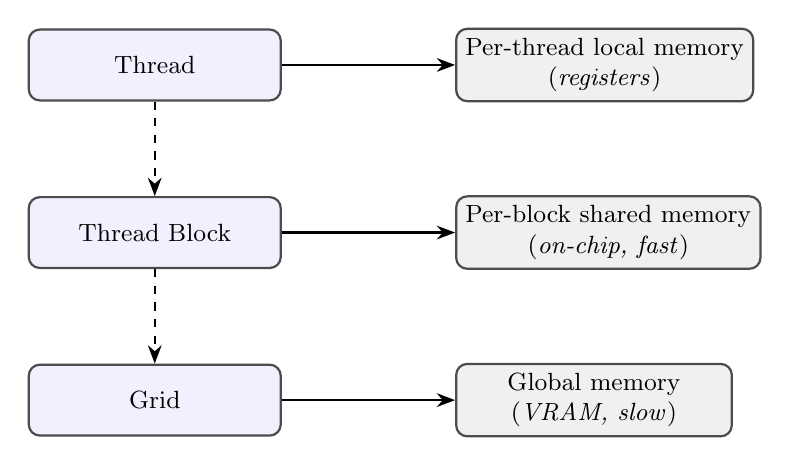
\begin{tikzpicture}[
  node distance=1.2cm,
  box/.style={rectangle, rounded corners, draw=black!70, thick, fill=blue!6,
              minimum width=3.2cm, minimum height=0.9cm, align=center, font=\small},
  mem/.style={rectangle, rounded corners, draw=black!70, thick, fill=gray!12,
              minimum width=3.5cm, minimum height=0.9cm, align=center, font=\small},
  arrow/.style={-Stealth, thick}
]
  \node[box] (thread) {Thread};
  \node[box, below=of thread] (block) {Thread Block};
  \node[box, below=of block] (grid) {Grid};

  \node[mem, right=2.2cm of thread] (local) {Per-thread local memory\\(\textit{registers})};
  \node[mem, right=2.2cm of block] (shared) {Per-block shared memory\\(\textit{on-chip, fast})};
  \node[mem, right=2.2cm of grid] (global) {Global memory\\(\textit{VRAM, slow})};

  \draw[arrow] (thread) -- (local);
  \draw[arrow] (block) -- (shared);
  \draw[arrow] (grid) -- (global);

  \draw[arrow, dashed] (thread) -- (block);
  \draw[arrow, dashed] (block) -- (grid);
\end{tikzpicture}
\end{center}

\begin{principle}[The fundamental asymmetry]
On a high-end accelerator the streaming multiprocessor (SM) may operate
roughly an order of magnitude faster than the VRAM that feeds it. A
typical datacentre card today carries $80~\text{GB}$ of VRAM but only
around $228~\text{KB}$ of on-chip SM memory per block. The consequence is
stark: if a computation must repeatedly consult VRAM, the arithmetic units
will spend most of their cycles idle, waiting.
\end{principle}

\subsection{Compute-Bound versus Memory-Bound}

This asymmetry gives rise to the single most important dichotomy in
inference engineering.

\begin{definition}[Compute-bound vs.\ memory-bound]
A computation is \textbf{compute-bound} if its wall-clock time is
dominated by arithmetic: reducing the number of floating-point operations
(FLOPs) reduces the total time. It is \textbf{memory-bound} if its
wall-clock time is dominated by data movement: reducing the volume of
bytes transferred between VRAM and the SM reduces the total time.
\end{definition}

A compute-bound kernel saturates the Tensor cores; a memory-bound kernel
leaves them idle while waiting for operands. The goal of inference
engineering is, almost universally, to move workloads from the
memory-bound regime into the compute-bound regime---or, when that is
impossible, to reduce the volume of memory traffic so severely that the
imbalance no longer matters.

\subsection{Aggregate Metrics: RPS, Latency, and the Compute Budget}

At the level of a deployed service, two numbers govern everything:

\begin{itemize}[leftmargin=1.5em, itemsep=2pt]
  \item \textbf{Requests per second (RPS)}---a measure of
        \emph{throughput}: how many requests the system completes per
        unit time.
  \item \textbf{Latency}---a measure of \emph{delay}: the time to complete
        a single request, typically reported in milliseconds.
\end{itemize}

These quantities are in perpetual tension. A service that maximises RPS by
batching aggressively will sacrifice latency; a service that minimises
latency by running single requests in isolation will leave most of its
hardware idle. The practitioner's art lies in finding the point on this
trade-off appropriate to the business.

\begin{remark}[On realistic traffic]
Stated load targets---``2000 RPS''---are projections, not observations.
Real traffic exhibits strong \emph{seasonality} (daily and weekly cycles)
and sudden spikes driven by external events (a new customer, a product
launch, a news cycle). A robust system must accommodate loads that may
vary from $10^2$ to $10^4$ RPS, not a single static figure. Cited latency
targets from competitors (``users waiting $>10$ seconds per token'') are
cautionary tales, not aspirations.
\end{remark}

\subsection{A Worked Example: Capacity Planning}

Consider a service with nominal load $2\text{K}$ RPS and a hard latency
budget of $<3$ seconds per request. Caching at a $20\%$ hit rate reduces
the effective demand:
\[
\text{average load} = 0.8 \cdot 2\text{K} = 1.6\text{K}~\text{RPS}, \qquad
\text{peak load} \approx 1.8\text{K}~\text{RPS}.
\]
Suppose each GPU in our fleet supports between $1$ and $6$ RPS (the range
reflects variation across prompt lengths). The required capacity is
approximately $300$ GPU-units; our provisioned budget is $200$. The
arithmetic is merciless:
\[
\underbrace{300}_{\text{demand}} \;>\; \underbrace{200}_{\text{budget}}
\quad\Longrightarrow\quad \text{system failure}.
\]
Bridging this gap is precisely the problem these lectures address.

\subsection{The Pareto Frontier}

When multiple optimisations are available, one cannot meaningfully rank
them by a single number. The natural object is the \emph{Pareto
frontier}: the set of configurations for which no alternative is
simultaneously faster and more accurate.

\begin{center}
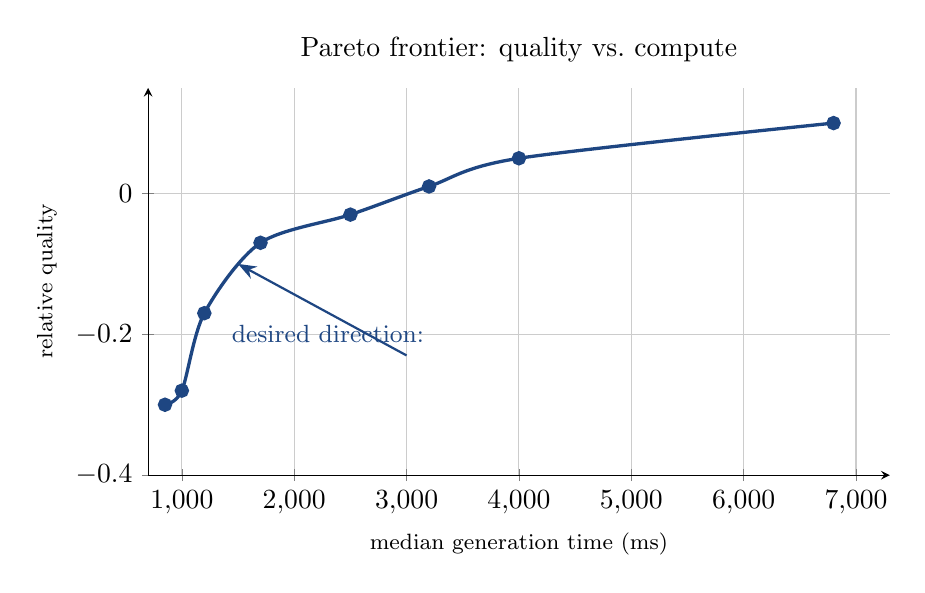
\begin{tikzpicture}
\begin{axis}[
    title={Pareto frontier: quality vs.\ compute},
    xlabel={median generation time (ms)},
    ylabel={relative quality},
    xmin=700, xmax=7300,
    ymin=-0.4, ymax=0.15,
    grid=both,
    major grid style={black!20},
    minor grid style={black!8},
    xtick={1000,2000,3000,4000,5000,6000,7000},
    width=11cm, height=6.5cm,
    axis lines=left,
    tick style={font=\footnotesize},
    label style={font=\footnotesize}
]
\addplot[accent, smooth, mark=*, very thick] coordinates {
  (850,-0.3) (1000,-0.28) (1200,-0.17) (1700,-0.07)
  (2500,-0.03) (3200,0.01) (4000,0.05) (6800,0.1)};
\node[accent, font=\small] at (axis cs:2300,-0.2) {desired direction:};
\draw[-Stealth, thick, accent] (axis cs:3000,-0.23) -- (axis cs:1500,-0.1);
\end{axis}
\end{tikzpicture}
\par\smallskip
{\small Schematic redraw of the slide's Pareto curve; the plotted values
are illustrative, not the original measurements.}
\end{center}

Each point on the curve represents a model configuration; the goal of
compression is to \emph{shift the curve leftward without shifting it
downward}. Increasing the density of available points gives the business a
richer menu of options, each suited to a different scenario (chat
interface, batch summarisation, offline evaluation).

\begin{principle}[Four questions for every compression technique]
\begin{enumerate}[leftmargin=1.8em, itemsep=2pt, label=\arabic*.]
  \item What does the $x$-axis represent---latency, or throughput?
  \item What quality metric anchors the $y$-axis?
  \item Where is the inflection point---the region of maximum return on
        investment?
  \item What is the compute budget, and does this technique fit inside it?
\end{enumerate}
\end{principle}

%%%%%%%%%%%%%%%%%%%%%%%%%%%%%%%%%%%%%%%%%%%%%%%%%%%%%%%%%%%%%%%%%%%%%%%%
\section{Transformer Inference: Two Phases, Two Regimes}
\label{sec:two-phases}
%%%%%%%%%%%%%%%%%%%%%%%%%%%%%%%%%%%%%%%%%%%%%%%%%%%%%%%%%%%%%%%%%%%%%%%%

Autoregressive generation in a transformer model decomposes naturally into
two phases. This decomposition is not merely pedagogical: the two phases
exhibit opposite computational profiles, and every serious optimisation
must distinguish between them.

\subsection{Context Processing (Prefill)}

Given an input prompt of length $L$, the model must first produce a rich
representation of every token. This phase is dominated by the scaled
dot-product attention,
\begin{equation}
  \operatorname{Attention}(Q, K, V) \;=\; \softmax\!\left(\frac{QK^\top}{\sqrt{d_k}}\right) V,
  \label{eq:attention}
\end{equation}
together with the surrounding feed-forward and projection layers.
Crucially, the entire sequence is processed in a single forward pass; the
operations reduce to \emph{general matrix multiplications} (GeMM), which
modern Tensor cores execute with near-peak efficiency.

\begin{remark}[Why prefill is compute-bound]
Let $L$ denote the context length, $d$ the hidden size, and consider the
$QK^\top$ computation: arithmetic scales as $\bigO(L^2 d)$, while memory
movement scales as $\bigO(L^2 + Ld)$. With $L$ in the thousands and $d$ in
the thousands, the arithmetic term dominates the memory term by roughly
three orders of magnitude---the same order separating SM throughput from
VRAM bandwidth. The phases cancel: prefill is comfortably compute-bound.
\end{remark}

Modern decoder-only architectures routinely handle contexts of
$128\text{K}$ tokens. The attention mask is \emph{causal} (triangular), so
each query attends only to itself and to prior keys. We will henceforth
refer to this phase simply as \emph{prefill}.

\subsection{Decoding}

Once the prompt has been processed, the model generates output tokens one
at a time. Each new token requires a full forward pass, but the query at
step $t$ is a single vector: the dominant operation is no longer
matrix--matrix but \emph{matrix--vector} multiplication (GeMV). The
arithmetic intensity---FLOPs per byte of memory movement---plummets.

\begin{center}
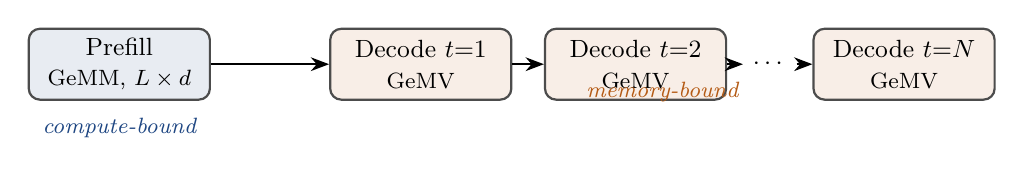
\begin{tikzpicture}[
  box/.style={rectangle, rounded corners, draw=black!70, thick,
              minimum width=2.3cm, minimum height=0.9cm, font=\small, align=center},
  prefill/.style={box, fill=accent!10},
  decode/.style={box, fill=remarkorange!10},
  arrow/.style={-Stealth, thick}
]
  \node[prefill] (pre) {Prefill\\\footnotesize GeMM, $L \times d$};
  \node[decode, right=1.5cm of pre] (d1) {Decode $t{=}1$\\\footnotesize GeMV};
  \node[decode, right=0.4cm of d1] (d2) {Decode $t{=}2$\\\footnotesize GeMV};
  \node[right=0.2cm of d2, font=\small] (dots) {$\cdots$};
  \node[decode, right=0.2cm of dots] (dn) {Decode $t{=}N$\\\footnotesize GeMV};

  \draw[arrow] (pre) -- (d1);
  \draw[arrow] (d1) -- (d2);
  \draw[arrow] (d2) -- (dots);
  \draw[arrow] (dots) -- (dn);

  \node[below=0.1cm of pre, font=\footnotesize\itshape, text=accent] {compute-bound};
  \node[below=0.1cm of $(d1)!0.5!(dn)$, font=\footnotesize\itshape, text=remarkorange] {memory-bound};
\end{tikzpicture}
\end{center}

\begin{principle}[The decoding bottleneck]
At decode time, every generated token requires loading the entire weight
matrix from VRAM. Because the GeMV performs only $\bigO(d)$ operations per
weight value (rather than the $\bigO(L)$ of GeMM), memory bandwidth
becomes the binding constraint. The decode phase is therefore
\emph{memory-bound}---and the Tensor cores sit mostly idle.
\end{principle}

\subsection{The KV Cache}

A naive implementation of autoregressive attention would recompute all
keys and values for the full prefix at every step---quadratic wastage. The
standard remedy is the \textbf{KV cache}: at step $t$, we store the
newly-computed $K_t$ and $V_t$, so that subsequent steps need only compute
the fresh query and attend to the accumulated cache.

Formally, at step $N$:
\begin{align}
  q_N &= W_Q x_N, \nonumber \\
  k_N &= W_K x_N, \quad v_N = W_V x_N, \nonumber \\
  K_{1:N} &= [\text{cached } K_{1:N-1};\, k_N], \quad V_{1:N} = [\text{cached } V_{1:N-1};\, v_N], \nonumber \\
  o_N &= \softmax\!\left(\frac{q_N K_{1:N}^\top}{\sqrt{d_k}}\right) V_{1:N}.
\end{align}
The cache converts quadratic work per token into linear work---at the cost
of a memory footprint that grows linearly in context length and batch
size. This cost will occupy much of our subsequent attention.

\subsection{Batching as Escape}

One way to escape the memory-bound regime of decoding is to \emph{batch}:
process many independent queries simultaneously, converting a GeMV back
into a GeMM. In the ideal case, batch size $\sim 1000$ restores
compute-boundedness. In practice, VRAM constraints---dominated by the KV
cache---sharply limit the achievable batch size. Batching is therefore a
genuine trade: throughput against memory.

%%%%%%%%%%%%%%%%%%%%%%%%%%%%%%%%%%%%%%%%%%%%%%%%%%%%%%%%%%%%%%%%%%%%%%%%
\section{Architectural Responses to the Decoding Bottleneck}
\label{sec:arch}
%%%%%%%%%%%%%%%%%%%%%%%%%%%%%%%%%%%%%%%%%%%%%%%%%%%%%%%%%%%%%%%%%%%%%%%%

\subsection{Rebalancing the Encoder--Decoder Ledger}

In classical encoder--decoder architectures (machine translation,
summarisation, retrieval-augmented generation), input and output are
handled by separate stacks. The encoder is run once per request; the
decoder is run once per generated token. If the decoder bears the bulk of
the parameters, every token pays that bulk.

A standard optimisation is to invert the usual budget---pushing perhaps
$70\%$ of the model's capacity into the encoder and leaving only $30\%$
for the decoder. Since the encoder runs once, its cost amortises over the
entire output; since the decoder runs many times, keeping it lean yields
large savings. Cross-attention provides the decoder selective access to
the encoder's rich representation:

\begin{center}
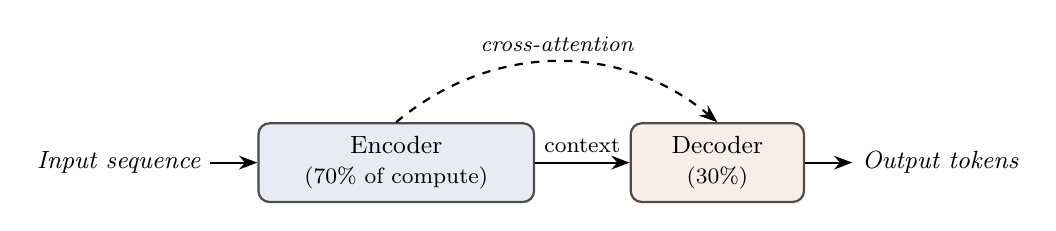
\begin{tikzpicture}[
  box/.style={rectangle, rounded corners, draw=black!70, thick,
              minimum height=1cm, align=center, font=\small},
  enc/.style={box, fill=accent!10, minimum width=3.5cm},
  dec/.style={box, fill=remarkorange!10, minimum width=2.2cm},
  io/.style={font=\small\itshape},
  arrow/.style={-Stealth, thick}
]
  \node[io] (in) {Input sequence};
  \node[enc, right=0.6cm of in] (enc) {Encoder\\\footnotesize (70\% of compute)};
  \node[dec, right=1.2cm of enc] (dec) {Decoder\\\footnotesize (30\%)};
  \node[io, right=0.6cm of dec] (out) {Output tokens};

  \draw[arrow] (in) -- (enc);
  \draw[arrow] (enc) -- node[above, font=\footnotesize] {context} (dec);
  \draw[arrow] (dec) -- (out);
  \draw[arrow, dashed, bend left=40] (enc.north) to node[above, font=\footnotesize\itshape] {cross-attention} (dec.north);
\end{tikzpicture}
\end{center}

The resulting system delivers the quality of a large model at the
inference speed of a small one---at least for context-heavy tasks where
the input is meaningfully longer than the output.

\subsection{Grouping the Heads: MHA, GQA, MQA}

A second lever acts directly on the KV cache rather than the weights.
Recall that standard \emph{multi-head attention} (MHA) maintains one $K$
and one $V$ projection per head; for a model with $h$ heads this
multiplies the cache size by $h$. \textbf{Multi-Query Attention}
(MQA)\footnote{N.\ Shazeer, ``Fast Transformer Decoding: One Write-Head is
All You Need'' (2019), \arxivlink{1911.02150}.} collapses all heads onto a
single shared $K,V$ pair; \textbf{Grouped-Query Attention}
(GQA)\footnote{J.\ Ainslie et al., ``GQA: Training Generalized Multi-Query
Transformer Models from Multi-Head Checkpoints'' (2023),
\arxivlink{2305.13245}.} interpolates by sharing $K,V$ within $g$ groups
of heads, $1 \le g \le h$.

\begin{definition}[KV-cache footprint]
For a model with $n_{\text{layer}}$ layers, head dimension $d_h$, $g$
key-value groups, batch size $bs$, sequence length $L$, and $\beta$ bytes
per scalar, the cache occupies
\begin{equation}
  M_{\text{KV}} \;=\; 2 \cdot n_{\text{layer}} \cdot g \cdot d_h \cdot bs \cdot L \cdot \beta,
  \label{eq:kv-size}
\end{equation}
the factor $2$ accounting for both $K$ and $V$. Reducing $g$ from $h$
(MHA) to a small group count, or to $g=1$ (MQA), shrinks $M_{\text{KV}}$
by exactly the factor $h/g$ with \emph{no} change to the FLOP count of the
forward pass---the projections $W_Q$ still produce $h$ query heads, only
the keys and values are shared.
\end{definition}

\begin{center}
\renewcommand{\arraystretch}{1.25}
\begin{tabular}{@{}lll@{}}
\toprule
\textbf{Variant} & \textbf{K/V arrangement} & \textbf{KV-cache size} \\
\midrule
Multi-Head Attention (MHA)    & One $K,V$ per head                  & $h \times$ baseline \\
Grouped-Query Attention (GQA) & One $K,V$ per group of heads        & $g \times$ baseline, $g < h$ \\
Multi-Query Attention (MQA)   & One $K,V$ shared across all heads   & $1 \times$ baseline \\
\bottomrule
\end{tabular}
\end{center}

GQA occupies the sweet spot: enough key-value diversity to preserve
quality (each group still specialises), but cache savings close to MQA's.
Because decoding is memory-bound (Section~\ref{sec:two-phases}), shrinking
$M_{\text{KV}}$ by a factor of $h/g$ is not a cosmetic change---it is a
direct, proportional reduction in the dominant cost of every decoding
step, and it is why GQA is the default in essentially every modern
open-weight model.

\subsection{Mixture of Experts}

If grouping queries controls the cache, \emph{Mixture of Experts}
(MoE)\footnote{W.\ Fedus, B.\ Zoph, N.\ Shazeer, ``Switch Transformers:
Scaling to Trillion Parameter Models with Simple and Efficient Sparsity''
(2021), \arxivlink{2101.03961}.} controls the weights. The standard dense
feed-forward network is replaced by a collection of $E$ parallel
``experts'', only $k \ll E$ of which are active for any given token. A
small router network selects the top-$k$ experts per token:
\begin{equation}
  y \;=\; \sum_{i=1}^{k} G(x)_i \, E_i(x),
  \label{eq:moe}
\end{equation}
where $G(x) \in \R^E$ is a sparse gating vector produced by $\softmax$
over the router's logits, and $E_i$ is the $i$-th expert's feed-forward
network.

\begin{center}
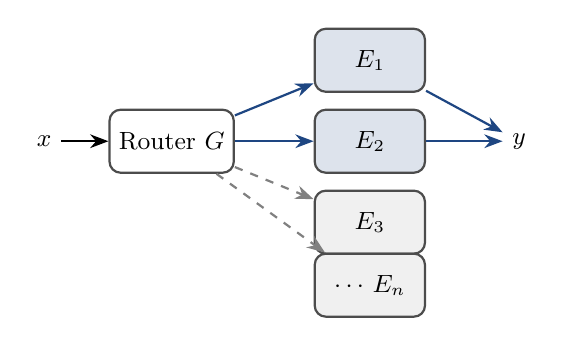
\begin{tikzpicture}[
  every node/.style={font=\small},
  expert/.style={rectangle, rounded corners, draw=black!70, thick,
                 minimum width=1.4cm, minimum height=0.8cm},
  active/.style={expert, fill=accent!15},
  inactive/.style={expert, fill=gray!12},
  arrow/.style={-Stealth, thick}
]
  \node (x) {$x$};
  \node[rectangle, rounded corners, draw=black!70, thick, right=0.6cm of x, minimum height=0.8cm] (router) {Router $G$};
  \draw[arrow] (x) -- (router);

  \node[active, above right=0.2cm and 1cm of router] (e1) {$E_1$};
  \node[active, right=1cm of router] (e2) {$E_2$};
  \node[inactive, below right=0.2cm and 1cm of router] (e3) {$E_3$};
  \node[inactive, below right=1cm and 1cm of router] (e4) {$\cdots\,E_n$};

  \draw[arrow, accent] (router) -- (e1);
  \draw[arrow, accent] (router) -- (e2);
  \draw[arrow, dashed, gray] (router) -- (e3);
  \draw[arrow, dashed, gray] (router) -- (e4);

  \node[right=3.4cm of router] (y) {$y$};
  \draw[arrow, accent] (e1) -- (y);
  \draw[arrow, accent] (e2) -- (y);
\end{tikzpicture}
\end{center}

The promise is to increase the total parameter count---and hence the
knowledge capacity---of the model without increasing the per-token
arithmetic cost: FLOPs scale with $k$, not $E$. The challenge, as we shall
see, is that MoE creates new and subtle load-balancing problems both at
training time and at inference time.

\begin{remark}[Load balancing during training]
Without intervention, the router collapses onto a small subset of
``favourite'' experts, starving the rest of gradient signal. The standard
fix, following the Switch Transformer formulation, adds an auxiliary loss
that penalises uneven routing:
\begin{equation}
  \mathcal{L}_{\text{aux}} \;=\; \lambda \cdot E \cdot \sum_{i=1}^{E} f_i \, P_i,
  \label{eq:moe-aux}
\end{equation}
where $f_i$ is the empirical fraction of tokens in the batch routed to
expert $i$ and $P_i$ is the router's average softmax probability mass on
expert $i$. The product $f_i P_i$ is minimised, for fixed total mass, when
routing is uniform across experts, so $\mathcal{L}_{\text{aux}}$ acts as a
soft constraint pulling the router toward balanced utilisation; $\lambda$
is a small coefficient (typically $10^{-2}$) chosen so the auxiliary term
does not dominate the primary language-modelling loss. This training-time
balancing is a prerequisite for the inference-time batching argument
below: a router that has learned to specialise unevenly will produce
exactly the imbalanced expert-batch sizes that defeat Tensor-core
utilisation.
\end{remark}

\subsection{MoE at Inference: The Expert-Batch Problem}

Suppose a model uses $E = 128$ experts with $k = 8$ active per token---a
sparsity ratio of $k/E = 1/16$. If the global inference batch is of size
$bs$, the expected number of tokens routed to any single expert is
\begin{equation}
  bs_{\text{expert}} \;=\; bs \cdot \frac{k}{E} \;=\; \frac{bs}{16}.
\end{equation}
Empirically, Tensor cores begin to approach their peak throughput only
when $bs_{\text{expert}} \gtrsim 128$. The implication is immediate:
\begin{equation}
  bs \;\geq\; 128 \times 16 \;=\; 2048.
\end{equation}

\begin{remark}[Empirical utilisation]
The dependence is sharply nonlinear. Measured Tensor-core utilisation for
a DeepSeek-V3-class MoE configuration:
\begin{center}
\renewcommand{\arraystretch}{1.25}
\begin{tabular}{@{}rr@{}}
\toprule
\textbf{Tokens per expert} & \textbf{Tensor-core utilisation} \\
\midrule
8   & 30--33\% \\
16  & 30--33\% \\
32  & 30--33\% \\
64  & 30--33\% \\
128 & 30--33\% \\
129 & 66\% \\
256 & 66\% \\
257 & 73--75\% \\
\bottomrule
\end{tabular}
\end{center}
The jump from $128$ to $129$ is an artefact of kernel tiling: the
hardware's natural work unit crosses a threshold. One reads this table as
follows: below the threshold, the expensive Tensor cores are idle most of
the time; above it, they earn their silicon.
\end{remark}

\subsection{The KV-Cache Memory Tension}

The compute argument demands large global batches; the memory argument
forbids them. For a single sample at sequence length $17\text{K}$ in BF16,
the KV cache occupies roughly $3~\text{GB}$. A batch of $1000$ samples
thus demands
\begin{equation}
  1000 \times 3~\text{GB} \;=\; 3~\text{TB of VRAM},
\end{equation}
well beyond any single node. MoE deployment is therefore a fundamentally
adversarial optimisation: the batch size that keeps experts compute-bound
is precisely the batch size that breaks the memory budget. The techniques
of subsequent sections---cache compression, offloading,
quantization---exist in large part to resolve this tension.

\subsection{Linear Attention and State-Space Models}

A more radical response abandons quadratic attention altogether.
\emph{State-space models} (SSMs) maintain a fixed-size internal state of
shape $d_{\text{hidden}} \times d_{\text{hidden}}$ and update it linearly
as tokens stream in. The result is an architecture whose memory and
arithmetic both scale \emph{linearly} in sequence length. A representative
family of such architectures includes Mamba, GatedDeltaNet, and the
linear-attention blocks of Qwen~3-Next, to which we return in
Section~\ref{sec:linear}.

%%%%%%%%%%%%%%%%%%%%%%%%%%%%%%%%%%%%%%%%%%%%%%%%%%%%%%%%%%%%%%%%%%%%%%%%
\section{VRAM Accounting and the Basics of Quantization}
\label{sec:quant-basics}
%%%%%%%%%%%%%%%%%%%%%%%%%%%%%%%%%%%%%%%%%%%%%%%%%%%%%%%%%%%%%%%%%%%%%%%%

Before introducing any clever compression scheme, we must account honestly
for where the memory goes. On a given GPU the budget equation is simply
\begin{equation}
  \underbrace{\text{weights}}_{\text{fixed per model}} \;+\;
  \underbrace{\text{KV cache}}_{\propto bs \cdot L} \;+\;
  \underbrace{\text{scratch/activations}}_{\propto bs} \;\leq\;
  \text{VRAM available}.
  \label{eq:vram-budget}
\end{equation}
As an illustration, a representative $8 \times 200$ configuration (eight
GPUs, $200~\text{GB}$ class; numbers in gigabytes) might satisfy
\begin{equation}
  470 + 3.05 \cdot bs + 20 \;\leq\; 1128 \quad\Longrightarrow\quad bs \leq 209,
\end{equation}
whereas an older $8 \times 100$ configuration permits only $bs \leq 49$.
Every gigabyte saved on weights or cache translates directly into headroom
for a larger batch---and hence higher throughput.

\subsection{Quantization as a Map to the Integer Grid}

\begin{definition}[Uniform quantization and dequantization]
Let $\mathbf{x} \in \R$ be a real-valued tensor entry. Fix a scale
$s > 0$, a zero-point $z \in \mathbb{Z}$, and a bit width $b$. The
\textbf{quantization} of $\mathbf{x}$ is
\begin{equation}
  \mathbf{x}^{(q)} \;=\; \clip\!\left(\left\lfloor \frac{\mathbf{x}}{s} \right\rfloor + z;\; 0,\; 2^b - 1\right),
  \label{eq:quant}
\end{equation}
and the corresponding \textbf{dequantization} is
\begin{equation}
  \hat{\mathbf{x}} \;=\; s \cdot (\mathbf{x}^{(q)} - z) \;\approx\; \mathbf{x}.
  \label{eq:dequant}
\end{equation}
The operation is intrinsically lossy: the floor and clip discard
information that cannot be recovered. In \emph{symmetric} quantization one
fixes $z = 0$, restricting the grid to be symmetric about the origin and
simplifying subsequent arithmetic.
\end{definition}

\subsection{Quantized Matrix Multiplication}

The practical use of quantization lies in the basic linear layer
$\mathbf{Y} = \mathbf{X}\mathbf{W}^\top$. If we quantize both operands,
\begin{align}
  \mathbf{X}^{(q)} &= \operatorname{quantize}(\mathbf{X};\, s_X, z_X), \\
  \mathbf{W}^{(q)} &= \operatorname{quantize}(\mathbf{W};\, s_W, z_W),
\end{align}
the core multiplication is performed entirely in integer
arithmetic---substantially cheaper on dedicated hardware---and the result
is dequantized only at the end. Schematically:

\begin{center}
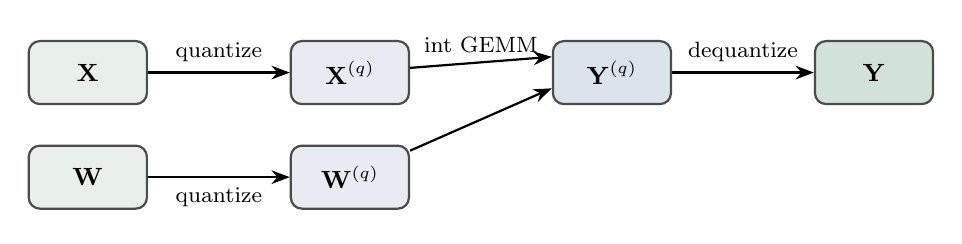
\begin{tikzpicture}[
  box/.style={rectangle, rounded corners, draw=black!70, thick,
              minimum width=1.5cm, minimum height=0.8cm, font=\small, align=center},
  arrow/.style={-Stealth, thick}
]
  \node[box, fill=defgreen!10] (X) {$\mathbf{X}$};
  \node[box, fill=defgreen!10, below=0.5cm of X] (W) {$\mathbf{W}$};
  \node[box, fill=accent!10, right=1.8cm of X] (Xq) {$\mathbf{X}^{(q)}$};
  \node[box, fill=accent!10, right=1.8cm of W] (Wq) {$\mathbf{W}^{(q)}$};
  \node[box, fill=accent!15, right=1.8cm of Xq] (Yq) {$\mathbf{Y}^{(q)}$};
  \node[box, fill=defgreen!20, right=1.8cm of Yq] (Y) {$\mathbf{Y}$};

  \draw[arrow] (X) -- node[above, font=\footnotesize] {quantize} (Xq);
  \draw[arrow] (W) -- node[below, font=\footnotesize] {quantize} (Wq);
  \draw[arrow] (Xq) -- node[above, font=\footnotesize] {int GEMM} ($(Yq.west)+(0,0.2)$);
  \draw[arrow] (Wq) -- ($(Yq.west)+(0,-0.2)$);
  \draw[arrow] (Yq) -- node[above, font=\footnotesize] {dequantize} (Y);
\end{tikzpicture}
\end{center}

The dequantized output recovers $\mathbf{Y}$ up to an error whose
magnitude depends on the choice of scales, the distribution of entries in
$\mathbf{X}$ and $\mathbf{W}$, and---crucially---the behaviour of
outliers.

\subsection{Taxonomy of Quantization Schemes}

Different practical regimes arise depending on \emph{what} is quantized
and \emph{when}:

\begin{itemize}[leftmargin=1.5em, itemsep=2pt]
  \item \textbf{Type 1 (Weight-only, \texttt{wNa16}):} Only weights are
        quantized; activations remain in FP16 or BF16. This minimises
        VRAM usage and accelerates the weight-loading memory traffic, but
        the actual GeMM is still performed in high precision.
  \item \textbf{Type 2 (\texttt{wNaM}):} Both weights and activations are
        quantized. This enables low-precision GEMM kernels (e.g.\ INT8 or
        FP8 Tensor-core paths) and can accelerate both memory transfer
        and computation.
  \item \textbf{Type 3 (Inflight):} Quantization is woven into the
        computation itself, produced and consumed on the fly rather than
        maintained as a static checkpoint attribute.
\end{itemize}

\begin{remark}[Cost of standard quantization]
Classical post-training quantization is cheap: a single host with a single
GPU and on the order of one thousand calibration examples usually
suffice, and quality loss is often negligible. A distinct and more
expensive family---\emph{quantization-aware training}---intertwines
quantization with the training loop itself and pays in compute what it
recovers in fidelity.
\end{remark}

%%%%%%%%%%%%%%%%%%%%%%%%%%%%%%%%%%%%%%%%%%%%%%%%%%%%%%%%%%%%%%%%%%%%%%%%
\section{GPT-Q: Weight-Only Quantization for Decoding}
\label{sec:gptq}
%%%%%%%%%%%%%%%%%%%%%%%%%%%%%%%%%%%%%%%%%%%%%%%%%%%%%%%%%%%%%%%%%%%%%%%%

GPT-Q\footnote{E.\ Frantar, S.\ Ashkboos, T.\ Hoefler, D.\ Alistarh,
``GPTQ: Accurate Post-Training Quantization for Generative Pre-trained
Transformers'' (2022), \arxivlink{2210.17323}.} is the first quantization
method of industrial consequence. Its contribution is twofold: a practical
algorithm for four-bit weight quantization that preserves quality, and---equally
important---an open-source release of optimised CUDA kernels that made the
method immediately deployable (it is highly popular in open source, and
underlies, for example, \texttt{llama.cpp} CPU inference).
Algorithmically, GPT-Q quantizes weights column by column, using a
second-order (Hessian-based) correction: after each column is rounded to
the grid, the resulting error is propagated to the remaining,
not-yet-quantized columns via the inverse of the layer's input covariance
matrix, so that later roundings partially compensate for earlier ones
rather than accumulating error independently.

\subsection{What GPT-Q Does}

GPT-Q targets the \texttt{W4A16} regime: four-bit weights, sixteen-bit
activations. The asymmetry is deliberate. Contemporary hardware does not
offer high-speed integer GEMM for four-bit activations, so there is no
gain to quantizing $\mathbf{X}$. But the weights of a large model dominate
the VRAM budget and their memory traffic dominates decode latency;
compressing them fourfold is exactly the intervention the memory-bound
regime demands.

A second deliberate choice: GPT-Q optimises \emph{decoding}, not prefill.
Since prefill is compute-bound and already saturates the Tensor cores,
there is no bandwidth bottleneck to relieve there.

\subsection{Practical Performance}

The original paper claimed speedups in the vicinity of $3.25\times$; in
production deployments the decoding-only speedup is typically $1.5\times$
to $2\times$---still substantial. The calibration (quantization) cost
itself is modest (the tables below are from the GPTQ paper, Tables~2 and
6):

\begin{center}
\renewcommand{\arraystretch}{1.25}
\begin{tabular}{@{}lcccc@{}}
\toprule
\textbf{Model} & OPT-13B & OPT-30B & OPT-66B & OPT-175B \\
\textbf{Runtime} & 20.9 min & 44.9 min & 1.6 h & 4.2 h \\
\midrule
\textbf{Model} & BLOOM-1.7B & BLOOM-3B & BLOOM-7.1B & BLOOM-176B \\
\textbf{Runtime} & 2.9 min & 5.2 min & 10.0 min & 3.8 h \\
\bottomrule
\end{tabular}
\end{center}

The per-token latency at batch size one (sequence length 128)
demonstrates the deployment impact:

\begin{center}
\renewcommand{\arraystretch}{1.25}
\begin{tabular}{@{}lcccc@{}}
\toprule
\textbf{GPU} & \textbf{FP16 latency} & \textbf{3-bit latency} & \textbf{Speedup} & \textbf{GPU reduction} \\
\midrule
A6000 (48 GB) & 589 ms & 130 ms & $4.53\times$ & $8 \to 2$ \\
A100 (80 GB)  & 230 ms & 71 ms  & $3.24\times$ & $5 \to 1$ \\
\bottomrule
\end{tabular}
\end{center}

The final column is the one that matters to a procurement officer:
quantization collapses the number of GPUs needed to host a given model,
often by factors of four or more.

\begin{remark}[On ``lossless'' claims]
Modern post-training quantization to four bits is often described as
lossless. The literature has, under careful evaluation, progressively
closed the gap: early techniques lost perhaps three to five percentage
points, while careful modern methods recover nearly all of it. One should
nevertheless regard ``lossless'' claims from community repositories (e.g.\
Hugging Face) with mild suspicion; the non-standardisation of quantization
pipelines means observed degradation varies widely between checkpoints.
\end{remark}

%%%%%%%%%%%%%%%%%%%%%%%%%%%%%%%%%%%%%%%%%%%%%%%%%%%%%%%%%%%%%%%%%%%%%%%%
\section{The Outlier Problem and the SmoothQuant Family}
\label{sec:smoothquant}
%%%%%%%%%%%%%%%%%%%%%%%%%%%%%%%%%%%%%%%%%%%%%%%%%%%%%%%%%%%%%%%%%%%%%%%%

When one attempts to quantize activations as well as weights---the
\texttt{W8A8} regime and its relatives---a new obstacle emerges.

\subsection{The Pathology of Activation Outliers}

Empirically, activations in transformer models exhibit sharp,
non-systematic spikes: occasional values whose magnitude dwarfs the rest of
the tensor. Because the quantization scale must accommodate the largest
value, these outliers dilate the grid and starve the bulk of the
distribution of precision.

The impact is sharply asymmetric between weights and activations. The
slides start from BERT: quantizing only the weights to 8 bits
(\texttt{W8A32}) leaves the GLUE average essentially unchanged ($83.23$
against $83.06$ for FP32), whereas quantizing only the activations
(\texttt{W32A8}) drops it to $70.25$---a loss of roughly thirteen points.
The same asymmetry persists at LLM scale. The table below shows
average zero-shot accuracy of OPT models of increasing size under three
INT8 activation-quantization granularities (the experiment is from the
SmoothQuant paper):

\begin{center}
\renewcommand{\arraystretch}{1.25}
\begin{tabular}{@{}lccccc@{}}
\toprule
\textbf{Model size (OPT)} & 6.7B & 13B & 30B & 66B & 175B \\
\midrule
FP16                 & 64.9\% & 65.6\% & 67.9\% & 69.5\% & 71.6\% \\
INT8 per-tensor      & 39.9\% & 33.0\% & 32.8\% & 33.1\% & 32.3\% \\
INT8 per-token       & 42.5\% & 33.0\% & 33.1\% & 32.9\% & 31.7\% \\
INT8 per-channel     & 64.8\% & 65.6\% & 68.0\% & 69.4\% & 71.4\% \\
\bottomrule
\end{tabular}
\end{center}

Per-channel quantization restores quality---but creates a fresh problem:
standard INT8 GEMM kernels do not support per-channel scales for
activations. The fast path and the accurate path are incompatible.

\begin{remark}[Why one cannot simply clip outliers]
A natural first reflex is to suppress outliers by clipping them or
replacing them with the mean. This is catastrophic: the top-$k$ output
probabilities collapse and the model effectively forgets how to
distinguish among its highest-confidence predictions. Outliers are not
noise; they are the signal. The craft of quantization lies in
\emph{coexisting} with them.
\end{remark}

\subsection{SmoothQuant: Migrating the Difficulty}

The central insight of SmoothQuant\footnote{G.\ Xiao, J.\ Lin, M.\ Seznec,
H.\ Wu, J.\ Demouth, S.\ Han, ``SmoothQuant: Accurate and Efficient
Post-Training Quantization for Large Language Models'' (2022),
\arxivlink{2211.10438}.} is that the product $\mathbf{X}\mathbf{W}^\top$
is invariant under the simultaneous transformation
\begin{equation}
  \mathbf{X} \mapsto \mathbf{X} \cdot \operatorname{diag}(s)^{-1}, \qquad
  \mathbf{W} \mapsto \mathbf{W} \cdot \operatorname{diag}(s).
  \label{eq:smooth-invariance}
\end{equation}
We can therefore transplant the outlier burden from the activations, where
it is crippling, onto the weights, where it is tolerable.

\begin{center}
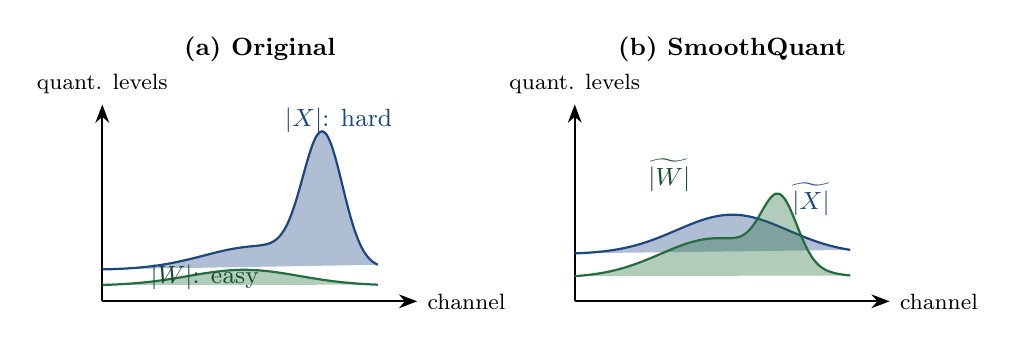
\begin{tikzpicture}[
  axis/.style={-Stealth, thick},
  dist/.style={thick, fill opacity=0.35},
  every node/.style={font=\small}
]
  % Original
  \begin{scope}
    \node[font=\small\bfseries] at (2, 3.2) {(a) Original};
    \draw[axis] (0,0) -- (0,2.5) node[above, font=\footnotesize] {quant. levels};
    \draw[axis] (0,0) -- (4,0) node[right, font=\footnotesize] {channel};
    \draw[dist, draw=accent, fill=accent] plot[smooth, domain=0:3.5, samples=60] (\x, {0.4 + 0.3*exp(-(\x-2)*(\x-2))+ 1.6*exp(-8*(\x-2.8)*(\x-2.8))});
    \node[accent] at (3.0, 2.3) {$|X|$: hard};
    \draw[dist, draw=defgreen, fill=defgreen] plot[smooth, domain=0:3.5, samples=60] (\x, {0.2 + 0.2*exp(-(\x-1.8)*(\x-1.8))});
    \node[defgreen!70!black] at (1.3, 0.3) {$|W|$: easy};
  \end{scope}

  % SmoothQuant
  \begin{scope}[xshift=6cm]
    \node[font=\small\bfseries] at (2, 3.2) {(b) SmoothQuant};
    \draw[axis] (0,0) -- (0,2.5) node[above, font=\footnotesize] {quant. levels};
    \draw[axis] (0,0) -- (4,0) node[right, font=\footnotesize] {channel};
    \draw[dist, draw=accent, fill=accent] plot[smooth, domain=0:3.5, samples=60] (\x, {0.6 + 0.5*exp(-(\x-2)*(\x-2))});
    \node[accent] at (3.0, 1.3) {$\widetilde{|X|}$};
    \draw[dist, draw=defgreen, fill=defgreen] plot[smooth, domain=0:3.5, samples=60] (\x, {0.3 + 0.5*exp(-(\x-1.8)*(\x-1.8)) + 0.8*exp(-10*(\x-2.6)*(\x-2.6))});
    \node[defgreen!70!black] at (1.2, 1.6) {$\widetilde{|W|}$};
  \end{scope}
\end{tikzpicture}
\end{center}

Activations become smooth and easy to quantize; weights become a little
harder, but since weights were easy to begin with they can absorb the
extra difficulty. The trade is almost always favourable.

\subsection{Choosing the Scale: Migration Strength $\alpha$}

The scale $s_j$ for channel $j$ is parameterised by a \emph{migration
strength} $\alpha \in [0,1]$:
\begin{equation}
  s_j \;=\; \frac{\max(|X_j|)^{\alpha}}{\max(|W_j|)^{1-\alpha}}.
  \label{eq:alpha}
\end{equation}
The extreme cases are
\begin{align*}
  \alpha \to 1 \quad&\text{(hard $W$, easy $A$):} \quad s_j \to \max(|X_j|), \\
  \alpha \to 0 \quad&\text{(easy $W$, hard $A$):} \quad s_j \to 1/\max(|W_j|),
\end{align*}
and the balanced regime sits between. A grid search over $\alpha$---performed
once, on a small calibration set---locates the sweet spot. For OPT-175B,
the optimal $\alpha$ preserves \texttt{W8A8} accuracy essentially at the
FP16 baseline.

\begin{principle}[Migration as a design principle]
SmoothQuant spawned an entire lineage of methods that relocate
quantization difficulty between operands. The general recipe is: find a
mathematically invariant transformation of the computation; use that
invariance to shift the hardest parts of the distribution into the
components best equipped to bear them. The rotation-based methods of the
next section take this principle to its natural conclusion.
\end{principle}

\subsection{Expected Gains and Overheads}

In practice, honest INT8 quantization of attention layers yields a
decoding speedup in the vicinity of $1.3\times$. Published claims of
$1.6\times$ or more usually rest either on a weak baseline or on a
configuration that hides the overhead of the quantize/dequantize
operations themselves. Any serious benchmark must account for these
auxiliary costs---the GEMM is not the whole story, and ignoring the
wrappers inflates the reported speedup.

%%%%%%%%%%%%%%%%%%%%%%%%%%%%%%%%%%%%%%%%%%%%%%%%%%%%%%%%%%%%%%%%%%%%%%%%
\section{FP8: When Hardware Catches Up with the Distribution}
\label{sec:fp8}
%%%%%%%%%%%%%%%%%%%%%%%%%%%%%%%%%%%%%%%%%%%%%%%%%%%%%%%%%%%%%%%%%%%%%%%%

The SmoothQuant approach is a software answer to a distributional problem.
The Hopper generation of GPUs offered a complementary hardware answer:
\emph{FP8 Tensor cores}\footnote{P.\ Micikevicius et al., ``FP8 Formats
for Deep Learning'' (2022), \arxivlink{2209.05433}.}. An FP8 number
carries a sign bit, a few exponent bits, and a few mantissa bits; the
exponent allows the format to gracefully span several orders of magnitude
of dynamic range, which is precisely what a distribution with outliers
requires. The slides' overview of FP8 quantization cites
\href{https://arxiv.org/pdf/2309.14592}{arXiv:2309.14592}.

\subsection{Why FP8 Helps}

Consider a tensor $X \sim \mathcal{N}(0, 0.5)$ contaminated with $1\%$
outliers uniform on $[-6, 6]$. Mapping to INT8---a uniform grid---forces a
trade: either the outliers are clipped, or the bulk of the distribution is
allocated few bins. FP8 variants (notably \texttt{E4M3} and \texttt{E5M2})
place their grid non-uniformly, devoting more precision to the common
region and accepting coarser resolution for the tails.

The quantization error, measured by
\begin{equation}
  \text{MSE} \;=\; \frac{1}{N}\sum_{i=1}^{N} (x_i - \hat{x}_i)^2,
\end{equation}
is consequently an order of magnitude smaller for \texttt{E4M3} than for
INT8 on such distributions.

\subsection{Simpler Scaling, Comparable Quality}

A significant practical virtue of FP8 is that \emph{per-tensor} scaling---one
scalar for the entire weight matrix---is usually sufficient. The
non-uniform grid absorbs much of what SmoothQuant had to accomplish
through channel-wise rescaling. Deployment is correspondingly simpler, and
typical speedups are on the order of $1.4\times$ over FP16---roughly
$10\%$ better than SmoothQuant's INT8 path. The slides summarise the
benefits (simple static amax-scaling, the E5M2 and E4M3 formats, per-tensor
quantization of weights and activations, $2\times$ weight compression) with
reference to the
\href{https://github.com/NVIDIA/TensorRT-LLM/blob/main/docs/source/blogs/quantization-in-TRT-LLM.md}{TensorRT-LLM
quantization blog post}.

\begin{center}
\renewcommand{\arraystretch}{1.25}
\begin{tabular}{@{}lccc@{}}
\toprule
\textbf{Model} & \textbf{Batch size} & \textbf{FP8 vs.\ FP16 speedup} & \textbf{INT8-sq vs.\ FP16 speedup} \\
\midrule
GPT-J        & 1 & $1.40\times$ & $1.40\times$ \\
GPT-J        & 8 & $1.44\times$ & -- \\
LLaMA-2 7B   & 1 & $1.51\times$ & $1.47\times$ \\
LLaMA-2 7B   & 8 & $1.40\times$ & -- \\
\bottomrule
\end{tabular}
\end{center}

The accuracy preservation is impressive:

\begin{center}
\renewcommand{\arraystretch}{1.25}
\begin{tabular}{@{}lcccc@{}}
\toprule
\textbf{Model} & \textbf{Method} & \textbf{MMLU FP16} & \textbf{MMLU post-quant} & \textbf{Loss} \\
\midrule
Falcon-180B & FP8  & 70.4 & 70.3 & 0.14\% \\
Falcon-180B & INT8 & 70.4 & 69.8 & 0.85\% \\
Falcon-40B  & FP8  & 56.1 & 55.6 & 0.89\% \\
Falcon-40B  & INT8 & 56.1 & 54.7 & 2.50\% \\
LLaMA-2 70B & FP8  & 69.1 & 68.5 & 0.87\% \\
LLaMA-2 70B & INT8 & 69.1 & 67.2 & 2.75\% \\
MPT-30B     & FP8  & 47.5 & 47.4 & 0.21\% \\
MPT-30B     & INT8 & 47.5 & 46.8 & 1.47\% \\
\bottomrule
\end{tabular}
\end{center}

\subsection{FP8 for Attention and the KV Cache}

FP8 also halves the KV cache memory footprint---roughly $3.05~\text{GB}$
drops to $1.52~\text{GB}$ for a reference configuration. By
Equation~\eqref{eq:kv-size}, this is the same lever as GQA, applied to
precision $\beta$ rather than to head count $g$; the two compose
multiplicatively. The downstream effect is dramatic: batch size doubles,
RPS doubles in production, and overall throughput doubles with it.
Combined with FlashAttention-3's\footnote{J.\ Shah, G.\ Bikshandi,
Y.\ Zhang, V.\ Thakkar, P.\ Ramani, T.\ Dao, ``FlashAttention-3: Fast and
Accurate Attention with Asynchrony and Low-precision'' (2024),
\arxivlink{2407.08608}. Builds on FlashAttention (Dao et al., NeurIPS
2022) and FlashAttention-2 (Dao, 2023, \arxivlink{2307.08691}).} FP8
kernels, prefill for $32\text{K}$-token sequences accelerates by more than
$1.25\times$ while remaining, for practical purposes, lossless (quality
loss below half a percentage point).

\begin{center}
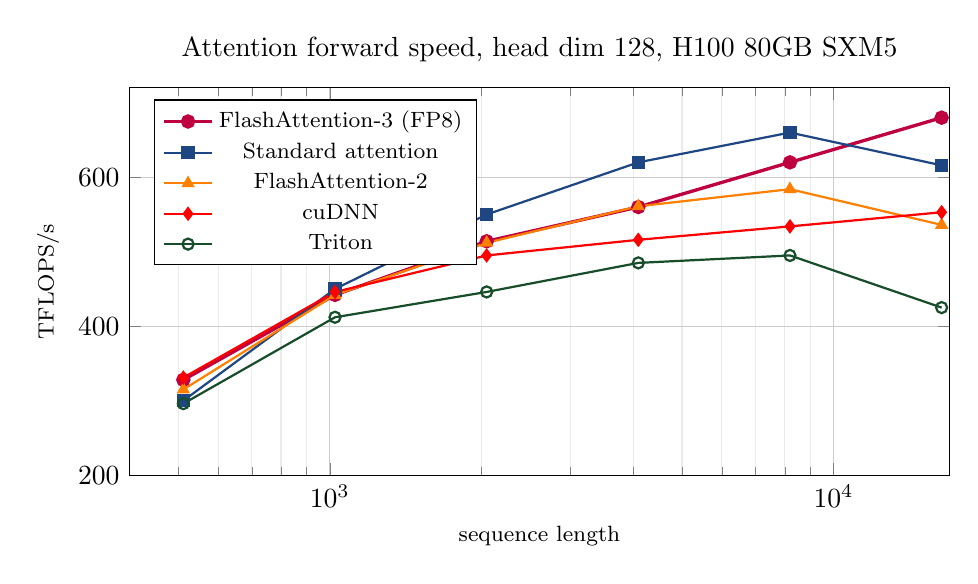
\begin{tikzpicture}
\begin{axis}[
    title={Attention forward speed, head dim 128, H100 80GB SXM5},
    xlabel={sequence length},
    ylabel={TFLOPS/s},
    xmin=400, xmax=17000,
    ymin=200, ymax=720,
    legend pos=north west,
    width=12cm, height=6.5cm,
    grid=both,
    major grid style={black!20},
    minor grid style={black!8},
    xmode=log,
    log basis x={10},
    tick style={font=\footnotesize},
    label style={font=\footnotesize},
    legend style={font=\footnotesize}
]
\addplot[purple, mark=*, very thick] coordinates {(512,328)(1024,442)(2048,514)(4096,560)(8192,620)(16384,680)};
\addlegendentry{FlashAttention-3 (FP8)}
\addplot[accent, mark=square*, thick] coordinates {(512,300)(1024,450)(2048,550)(4096,620)(8192,660)(16384,616)};
\addlegendentry{Standard attention}
\addplot[orange, mark=triangle*, thick] coordinates {(512,315)(1024,442)(2048,512)(4096,561)(8192,584)(16384,536)};
\addlegendentry{FlashAttention-2}
\addplot[red, mark=diamond*, thick] coordinates {(512,331)(1024,446)(2048,495)(4096,516)(8192,534)(16384,553)};
\addlegendentry{cuDNN}
\addplot[defgreen!70!black, mark=o, thick] coordinates {(512,296)(1024,412)(2048,446)(4096,485)(8192,495)(16384,425)};
\addlegendentry{Triton}
\end{axis}
\end{tikzpicture}
\par\smallskip
{\small Schematic redraw of the slide's plot; the plotted values are
approximate, not the original measurements.}
\end{center}

%%%%%%%%%%%%%%%%%%%%%%%%%%%%%%%%%%%%%%%%%%%%%%%%%%%%%%%%%%%%%%%%%%%%%%%%
\section{Rotations and the Geometry of Outliers: SpinQuant}
\label{sec:spinquant}
%%%%%%%%%%%%%%%%%%%%%%%%%%%%%%%%%%%%%%%%%%%%%%%%%%%%%%%%%%%%%%%%%%%%%%%%

SmoothQuant migrates outlier pain between tensors; FP8 accommodates
outliers by choosing a more forgiving grid. A third approach,
\textbf{SpinQuant}\footnote{Z.\ Liu et al., ``SpinQuant: LLM Quantization
with Learned Rotations'' (2024, ICLR 2025), \arxivlink{2405.16406}.},
attacks the geometry of the problem itself: rotate the tensor so that the
outliers disperse.

\subsection{The Geometric Picture}

Activation tensors of transformer models exhibit a characteristic
geometric signature. If one visualises the joint distribution of feature
dimensions as a point cloud, it tends to be highly \emph{anisotropic}:
elongated along a small number of axes (the outlier channels) and
compressed along the remainder. From a quantization standpoint, the
elongation is disaster; a uniform grid must accommodate the full length of
the major axis, wasting resolution on the many short axes.

\begin{center}
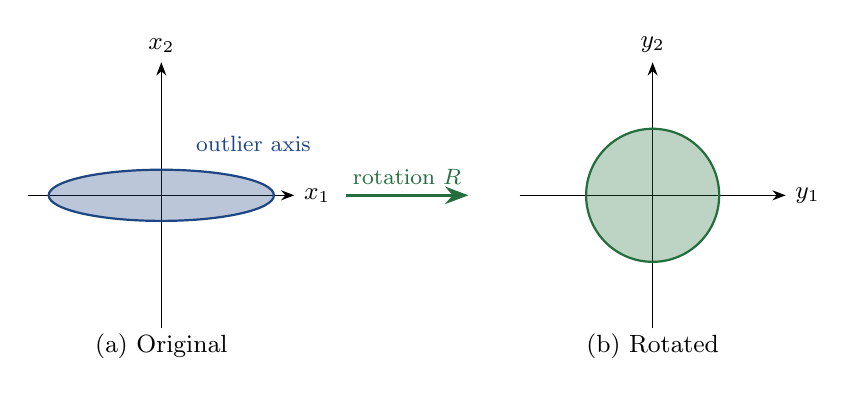
\begin{tikzpicture}[scale=1.3, every node/.style={font=\small}]
  \begin{scope}
    \draw[-Stealth, thin] (-1.3,0) -- (1.3,0) node[right] {$x_1$};
    \draw[-Stealth, thin] (0,-1.3) -- (0,1.3) node[above] {$x_2$};
    \draw[thick, accent, fill=accent, fill opacity=0.3] (0,0) ellipse (1.1 and 0.25);
    \node[below=0.6cm] at (0,-0.8) {(a) Original};
    \node[accent, font=\footnotesize] at (0.9, 0.5) {outlier axis};
  \end{scope}

  \draw[-Stealth, very thick, defgreen] (1.8,0) -- (3,0) node[midway, above, font=\footnotesize] {rotation $R$};

  \begin{scope}[xshift=4.8cm]
    \draw[-Stealth, thin] (-1.3,0) -- (1.3,0) node[right] {$y_1$};
    \draw[-Stealth, thin] (0,-1.3) -- (0,1.3) node[above] {$y_2$};
    \draw[thick, defgreen, fill=defgreen, fill opacity=0.3] (0,0) circle (0.65);
    \node[below=0.6cm] at (0,-0.8) {(b) Rotated};
  \end{scope}
\end{tikzpicture}
\end{center}

An orthogonal rotation is information-preserving but can redistribute
variance across axes. If we choose $R$ well, the result is isotropic:
every axis carries a manageable portion of the variance, and quantization
proceeds uneventfully.

\subsection{Kurtosis: A Scalar Summary of the Problem}

The ``outlier-ness'' of a distribution is captured quantitatively by the
kurtosis,
\begin{equation}
  \operatorname{Kurt}[X] \;=\; \E\!\left[\left(\frac{X-\mu}{\sigma}\right)^4\right] \;=\; \frac{\mu_4}{\sigma^4},
\end{equation}
where $\mu_4$ is the fourth central moment. A Gaussian has kurtosis $3$;
heavier-tailed distributions exceed it, sometimes dramatically.
Activations of an unrotated LLaMA-2 7B show persistently high and
unstable kurtosis; after the SpinQuant rotation, the kurtosis of every
layer collapses toward the Gaussian value, and quantization error drops
with it.

\subsection{The SpinQuant Recipe}

SpinQuant achieves stable \texttt{W4A4KV4} quantization---four bits for
weights, activations, and the KV cache simultaneously---through four
ingredients:

\begin{enumerate}[leftmargin=1.8em, itemsep=2pt]
  \item \textbf{Smooth with rotation.} Orthogonal rotations applied at
        strategic points in the residual stream redistribute outliers.
  \item \textbf{Learnable rotations.} The rotation matrices are not fixed
        but \emph{learned} on a calibration set, minimising quantization
        error. Optimisation on the Stiefel manifold of orthogonal matrices
        uses Cayley SGD, which preserves orthogonality at every step.
  \item \textbf{Fusion into weights.} Whenever a rotation sits adjacent to
        a linear layer, it is mathematically absorbed into the weight
        matrix. The fused layer is numerically equivalent but costs no
        extra inference time.
  \item \textbf{Hadamard rotations as fallback.} Where fusion is
        impossible---for instance, immediately after a non-linearity---a
        Hadamard matrix is used instead. Hadamard matrices admit an
        $\bigO(n \log n)$ multiplication and add negligible overhead.
\end{enumerate}

\subsection{Architectural Placement}

The residual stream of a standard transformer block is
\[
  \text{Embedding} \to \text{MHSA} \to \text{FFN} \to \text{Output},
\]
and SpinQuant inserts four rotations $R_1, R_2, R_3, R_4$:
\[
  \text{Embedding} \xrightarrow{R_1} \text{MHSA} \xrightarrow{R_2} \xrightarrow{R_3} \text{FFN} \xrightarrow{R_4} \text{Output}.
\]
Here $R_1$ and $R_2$ are typically merged into neighbouring linear layers;
$R_3$ handles the KV cache specifically; $R_4$ targets activation
quantization in the FFN.

\subsection{Learnable versus Fixed Rotations}

Why bother learning the rotation rather than using a random or Hadamard
rotation? Empirically, the answer is worth roughly three percentage points
of accuracy:

\begin{center}
\renewcommand{\arraystretch}{1.25}
\begin{tabular}{@{}lc@{}}
\toprule
\textbf{Rotation method} & \textbf{Zero-shot reasoning accuracy} \\
\midrule
Random                          & widest spread, lowest median \\
Hadamard (fixed)                & tighter, higher median \\
Cayley-optimised (learned)      & tightest, highest median \\
\bottomrule
\end{tabular}
\end{center}

The learned rotation finds a configuration adapted to the actual
activation distribution of the trained model; random or fixed rotations,
however elegant, cannot exploit this structure.

\begin{remark}[A cautionary note on scale]
Quality of quantization is not monotone in model size. Very large models
trained on very large datasets (e.g.\ $20~\text{T}$ tokens with
$1.3~\text{B}$ parameters) sometimes prove \emph{harder} to quantize than
their smaller or less-saturated siblings. The folk intuition---``larger
models have redundancy to spare''---is true only until it isn't. The
relevant quantity is not the parameter count alone but the parameter count
relative to the information pressure of the training data.
\end{remark}

%%%%%%%%%%%%%%%%%%%%%%%%%%%%%%%%%%%%%%%%%%%%%%%%%%%%%%%%%%%%%%%%%%%%%%%%
\section{Block Quantization: MXFP4 and NVFP4}
\label{sec:fp4}
%%%%%%%%%%%%%%%%%%%%%%%%%%%%%%%%%%%%%%%%%%%%%%%%%%%%%%%%%%%%%%%%%%%%%%%%

The frontier of numerical compression continues to advance. The most
recent generation of formats---MXFP4\footnote{Open Compute Project, ``OCP
Microscaling Formats (MX) Specification v1.0'' (2023),
\href{https://www.opencompute.org/documents/ocp-microscaling-formats-mx-v1-0-spec-final-pdf}{opencompute.org}.}
and NVFP4\footnote{NVIDIA, ``Introducing NVFP4 for Efficient and Accurate
Low-Precision Inference'' (2024),
\href{https://developer.nvidia.com/blog/introducing-nvfp4-for-efficient-and-accurate-low-precision-inference/}{developer.nvidia.com}.}---performs
\emph{block quantization}: rather than assigning one scale to an entire
row or column, the tensor is partitioned into contiguous blocks of 16 or
32 values, each with its own scale. The per-block overhead is modest (on
the order of $1\%$ extra storage) but the dynamic range is enormously
improved.

\subsection{Anatomy of the Formats}

Each FP4 value carries a sign bit $s$, exponent bits $e$, and mantissa
bits $m$. The surrounding scaling architecture differs:

\begin{center}
\renewcommand{\arraystretch}{1.25}
\begin{tabular}{@{}lll@{}}
\toprule
& \textbf{MXFP4} & \textbf{NVFP4} \\
\midrule
Block size           & 32 values                      & 16 values \\
Per-block scale      & E8M0                           & E4M3 \\
Per-tensor scale     & E8M0                           & FP32 (E8M23) \\
Accumulator          & FP8 (BF16 on high-end HW)      & FP8 (BF16 on high-end HW) \\
\bottomrule
\end{tabular}
\end{center}

NVFP4's two-level scaling---a rich per-block scale combined with a full
FP32 global scale---captures distributions with extreme dynamic range, and
is particularly effective at handling outliers without a separate rotation
step.

\subsection{Do We Still Need Hadamard Rotations?}

A subtle and important empirical finding: Hadamard rotations, so useful
for MXFP4, provide little benefit for NVFP4. The richer block-level
scaling of NVFP4 already absorbs the difficulty that rotations were
invented to address. In a production deployment of NVFP4 one may therefore
omit the rotation step entirely, fusing the weights into a simpler kernel
and streamlining the inference path.

This is an instructive episode. A technique that was essential in one
generation of formats becomes obsolete in the next---not because it was
wrong, but because hardware advanced to subsume it. The practitioner must
periodically re-examine which rungs of their engineering ladder are still
load-bearing.

%%%%%%%%%%%%%%%%%%%%%%%%%%%%%%%%%%%%%%%%%%%%%%%%%%%%%%%%%%%%%%%%%%%%%%%%
\section{Speculative Decoding: The Economy of Easy Tokens}
\label{sec:spec-dec}
%%%%%%%%%%%%%%%%%%%%%%%%%%%%%%%%%%%%%%%%%%%%%%%%%%%%%%%%%%%%%%%%%%%%%%%%

We now leave quantization behind and turn to a qualitatively different
idea. Observe a basic fact about autoregressive generation: most generated
tokens are \emph{easy}. Common function words, predictable continuations,
punctuation---the model assigns them near-unit probability, and any
reasonable approximation would produce the same choice. Only a small
fraction of tokens---roughly a quarter to a third---exercise the full
discriminative power of the large model.

Standard decoding pays the full cost of the large model on every token,
easy or hard. \textbf{Speculative decoding}\footnote{Y.\ Leviathan,
M.\ Kalman, Y.\ Matias, ``Fast Inference from Transformers via Speculative
Decoding'' (ICML 2023), \arxivlink{2211.17192}; independently, C.\ Chen
et al., ``Accelerating Large Language Model Decoding with Speculative
Sampling'' (2023), \arxivlink{2302.01318}.} pays the full cost only on
hard ones.

\subsection{The Basic Idea}

Introduce a small ``draft'' model $p$---fast but approximate---and keep the
expensive ``target'' model $q$---accurate but slow. At each step:

\begin{enumerate}[leftmargin=1.8em, itemsep=2pt]
  \item The draft model proposes $K$ tokens in quick succession.
  \item The target model processes the entire $K$-token draft in a single
        forward pass (a GeMM, not $K$ GeMVs).
  \item A stochastic acceptance test decides, token by token, which drafts
        to keep. If all $K$ are accepted, we have effectively generated
        $K$ tokens at the cost of one target-model forward pass plus $K$
        draft-model passes. If token $j$ is rejected, we correct it using
        the target model and restart from there.
\end{enumerate}

Consider a simple greedy example. From \texttt{[BOS]}, the draft proposes
``\texttt{She}, \texttt{enjoyed}, \texttt{the}, \texttt{quiet},
\texttt{morning}, \texttt{sipping}''. The target verifies each in
parallel. Where the draft and target agree, we accept. Where they
disagree---perhaps the draft proposes \texttt{sipping} but the target
prefers \texttt{evening}---we accept the target's choice and truncate the
speculation at that point.

\begin{center}
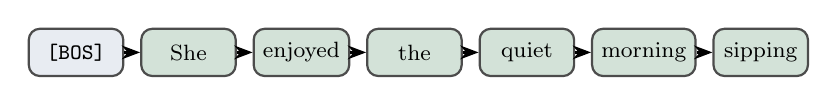
\begin{tikzpicture}[
  every node/.style={font=\footnotesize},
  tok/.style={rectangle, rounded corners, draw=black!70, thick,
              minimum width=1.2cm, minimum height=0.6cm, fill=accent!10},
  acc/.style={rectangle, rounded corners, draw=black!70, thick,
              minimum width=1.2cm, minimum height=0.6cm, fill=defgreen!20},
  arrow/.style={-Stealth, thick}
]
  \node[tok] (b) {\texttt{[BOS]}};
  \node[acc, right=0.2cm of b] (t1) {She};
  \node[acc, right=0.2cm of t1] (t2) {enjoyed};
  \node[acc, right=0.2cm of t2] (t3) {the};
  \node[acc, right=0.2cm of t3] (t4) {quiet};
  \node[acc, right=0.2cm of t4] (t5) {morning};
  \node[acc, right=0.2cm of t5] (t6) {sipping};
  \draw[arrow] (b) -- (t1);
  \draw[arrow] (t1) -- (t2);
  \draw[arrow] (t2) -- (t3);
  \draw[arrow] (t3) -- (t4);
  \draw[arrow] (t4) -- (t5);
  \draw[arrow] (t5) -- (t6);
\end{tikzpicture}
\end{center}

\subsection{Formal Algorithm}

\begin{theorem}[Speculative Sampling (SpS)]
Given a target model $q$, a draft model $p$, a speculation length $K$, and
a current context of length $n$, the following procedure produces samples
whose distribution is \emph{exactly} that of the target model $q$:

\begin{enumerate}[leftmargin=1.8em, itemsep=2pt]
  \item Draw $K$ draft tokens $x_{n+1}, \ldots, x_{n+K}$ autoregressively
        from $p$.
  \item Compute $q(x \mid x_{<n+t})$ for $t = 1, \ldots, K$ in a single
        target-model forward pass.
  \item For $t = 1, \ldots, K$ in order, draw $r \sim U[0,1]$ and
        \textbf{accept} $x_{n+t}$ iff
        \[
          r \;\leq\; \min\!\left(1,\; \frac{q(x_{n+t}\mid x_{<n+t})}{p(x_{n+t}\mid x_{<n+t})}\right).
        \]
  \item On the first rejection at position $t$, resample a correction
        $x_{n+t}$ from the residual
        \[
          x_{n+t} \;\sim\; \operatorname{norm}\!\bigl(\max\bigl(0,\; q(\cdot\mid x_{<n+t}) - p(\cdot\mid x_{<n+t})\bigr)\bigr),
        \]
        advance $n \gets n + t$, and return to step 1.
  \item If all $K$ are accepted, advance $n \gets n + K$ and return to
        step 1.
\end{enumerate}
\end{theorem}

The acceptance criterion is the ratio test of rejection sampling: it
ensures that the accepted samples are distributed exactly as $q$ would
distribute them, despite having been proposed by $p$. This is the deep
guarantee of speculative sampling: \textbf{it does not merely approximate
the target model; it samples from it exactly}.

\begin{remark}[Where does the speedup come from?]
The total amount of computation is, in the worst case, larger than
standard decoding: every speculation that fails is a unit of wasted work.
The speedup comes from \emph{memory-boundedness}. During decoding the
target-model weights must be loaded from VRAM; this memory traffic is
essentially the same whether we evaluate one token or six. If the batch of
six tokens can be formed by speculation, we have amortised one memory load
over six generated tokens. The latency of generating six tokens approaches
that of generating one.
\end{remark}

%%%%%%%%%%%%%%%%%%%%%%%%%%%%%%%%%%%%%%%%%%%%%%%%%%%%%%%%%%%%%%%%%%%%%%%%
\section{EAGLE: Speculative Decoding as Architecture}
\label{sec:eagle}
%%%%%%%%%%%%%%%%%%%%%%%%%%%%%%%%%%%%%%%%%%%%%%%%%%%%%%%%%%%%%%%%%%%%%%%%

The efficiency of speculative decoding hinges on a single quantity: the
\textbf{acceptance rate}---the expected fraction of drafted tokens that
survive verification. The higher the acceptance rate, the more tokens
generated per target-model forward pass, and the greater the speedup. The
question becomes: how should the draft model be constructed to maximise
alignment with the target?

The traditional answer---use a separately-trained small model of the same
family---is serviceable but suboptimal. The small model has never seen the
large model's internal representations; it must approximate them from the
outside. The \textbf{EAGLE} family\footnote{Y.\ Li, F.\ Wei, C.\ Zhang,
H.\ Zhang, ``EAGLE: Speculative Sampling Requires Rethinking Feature
Uncertainty'' (2024), \arxivlink{2401.15077}; ``EAGLE-2: Faster Inference
of Language Models with Dynamic Draft Trees'' (2024),
\arxivlink{2406.16858}; ``EAGLE-3: Scaling up Inference Acceleration of
Large Language Models via Training-Time Test'' (2025),
\arxivlink{2503.01840}.} reverses this: it makes the drafter not a
separate model but a lightweight \emph{head} on top of the target model's
frozen body.

\subsection{Architecture: The Drafter as Head}

A key motivating observation is that standard autoregressive generation
suffers from a \emph{distribution mismatch}: as the token chain deepens,
the model's outputs progressively diverge from its own internal
hypotheses, degrading generative coherence. EAGLE addresses this by
grounding the drafter in the target's own feature space.

Specifically, the EAGLE drafter consists of a single transformer layer
operating on the hidden states of the frozen target model. Its size is
roughly $1/48$ that of the target---negligible. The base model is kept
frozen during drafter training; only the drafter's one layer is optimised.

\begin{center}
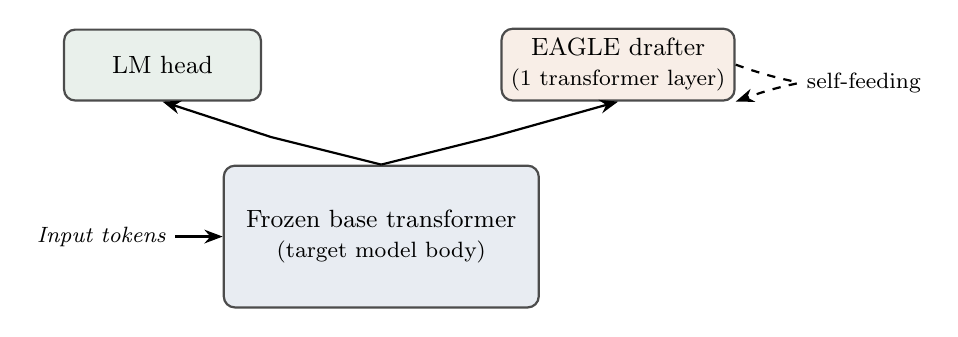
\begin{tikzpicture}[
  every node/.style={font=\small},
  body/.style={rectangle, rounded corners, draw=black!70, thick, fill=accent!10,
               minimum width=4cm, minimum height=1.8cm, align=center},
  head/.style={rectangle, rounded corners, draw=black!70, thick, fill=remarkorange!10,
               minimum width=2.5cm, minimum height=0.9cm, align=center},
  lm/.style={rectangle, rounded corners, draw=black!70, thick, fill=defgreen!10,
             minimum width=2.5cm, minimum height=0.9cm, align=center},
  arrow/.style={-Stealth, thick}
]
  \node[body] (base) {Frozen base transformer\\\footnotesize (target model body)};
  \node[lm, above left=0.8cm and -0.5cm of base] (lmhead) {LM head};
  \node[head, above right=0.8cm and -0.5cm of base] (drafter) {EAGLE drafter\\\footnotesize (1 transformer layer)};

  \draw[arrow] (base.north) -- ++(-1.4,0.35) -- (lmhead.south);
  \draw[arrow] (base.north) -- ++(1.4,0.35) -- (drafter.south);

  \node[left=0.6cm of base, font=\footnotesize\itshape] (in) {Input tokens};
  \draw[arrow] (in) -- (base);

  \draw[arrow, dashed] (drafter.east) to[out=-20, in=20, looseness=6] node[right, font=\footnotesize] {self-feeding} (drafter.south east);
\end{tikzpicture}
\end{center}

A critical implementation detail is \textbf{activation injection}: rather
than receiving only the final-layer hidden states, the EAGLE head is
injected with activations from one of the middle layers of the base model.
This allows the lightweight drafter to access rich contextual
representations at reduced cost---no reprocessing of the full layer stack
is required. The resulting component is called the
\textbf{FeatExtrapolator}: it projects these intermediate embeddings to
predict future hidden states before the base model formally computes them.

The benefit is conceptual: the drafter has direct access to the target's
internal representations. It is not guessing from surface form but
extrapolating from the same feature space the target will use to verify
its proposals. The result is an unusually high acceptance rate.

\subsection{Inference Mechanics: The Draft--Verify Loop}

To make the architecture concrete, consider generating the continuation of
``How can\ldots''. The full inference cycle proceeds as follows.

\begin{description}[leftmargin=1.5em, style=nextline]
  \item[Step 1 --- Target forward pass.] The frozen target LLM processes
    the existing context and produces two outputs: (a) the next accepted
    tokens (e.g.\ \texttt{can}, \texttt{I}) via sampling from the LM head,
    and (b) the corresponding final-layer hidden states
    $f_{\text{how}}, f_{\text{can}}$. These hidden states are injected
    into the drafter via a dashed residual connection; this is the
    activation injection described above.
  \item[Step 2 --- Drafter forward pass 1.] The drafter's single
    transformer layer receives \emph{pairs} $(f_i, e_i)$, where $f_i$ is
    the hidden state from the target and $e_i$ is the token embedding.
    Concretely it processes $(f_{\text{how}}, e_{\text{can}})$ and
    $(f_{\text{can}}, e_{\text{I}})$. Why pairs and not embeddings alone?
    The embedding $e_i$ encodes the surface identity of the token; the
    hidden state $f_i$ encodes the full contextual meaning as computed by
    the target. Together they give the drafter everything the target had
    when it produced that position. The drafter predicts the next hidden
    state $\tilde{f}_{\text{I}}$, which is passed through the (frozen) LM
    head to sample draft candidates---e.g.\ \texttt{make} and \texttt{help}
    in parallel (``sampling multiple times'').
  \item[Step 3 --- Drafter forward passes 2, 3, \ldots] The drafter now
    \emph{self-feeds}: it takes its own predicted $\tilde{f}_{\text{I}}$
    together with the embeddings of the sampled candidates
    $e_{\text{make}}, e_{\text{help}}$ and runs another forward pass,
    producing the next level of the draft tree. This is repeated for a
    fixed number of steps (typically 3). Crucially, no target model call
    is made during these steps; the cost is only one lightweight
    transformer layer per step, applied in parallel across all active
    branches.
  \item[Step 4 --- Target verification.] After $K$ drafter steps the full
    candidate tree is flattened and fed to the target LLM in a single
    forward pass. The target's logits reveal which branch it would have
    chosen; all tokens along the longest matching prefix are accepted.
    Tokens beyond the first mismatch are rejected, and the cycle restarts
    from the last accepted token.
\end{description}

The efficiency gain is immediate:

\begin{center}
\renewcommand{\arraystretch}{1.25}
\begin{tabular}{@{}lc@{}}
\toprule
\textbf{Scheme} & \textbf{Tokens per target forward pass} \\
\midrule
Vanilla autoregression & $1$ \\
EAGLE (3 drafter steps, top-2 tree) & ${\sim}3$--$4$ \\
\bottomrule
\end{tabular}
\end{center}

\begin{remark}[Why self-feeding degrades with depth]
At drafter step 1 the input hidden state $f$ is exact---it comes directly
from the target. At steps 2, 3, \ldots\ the drafter uses its own predicted
$\tilde{f}$, which carries approximation error. This error accumulates, so
acceptance rates fall as speculation depth $n$ grows. EAGLE-3 addresses
this by eliminating the explicit hidden-state modelling loss and fusing
features differently, as discussed in Section~\ref{ssec:eagle3}.
\end{remark}

\subsection{Tree-Structured Speculation}

A second EAGLE innovation is structural. Rather than proposing a single
linear sequence of $K$ tokens, the drafter generates a \emph{tree} of
alternative continuations via the FeatExtrapolator. At each step it
considers the top-$2$ candidates; the target model verifies the whole tree
in one forward pass, following whichever branch its top-1 predictions
trace out.

\begin{center}
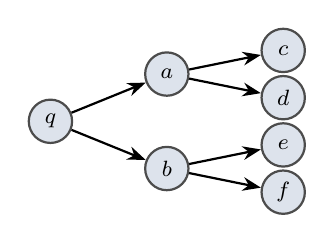
\begin{tikzpicture}[
  every node/.style={font=\footnotesize},
  tok/.style={circle, draw=black!70, thick, minimum size=0.55cm, inner sep=0pt, fill=accent!15},
  arrow/.style={-Stealth, thick}
]
  \node[tok] (r) {$q$};
  \node[tok, right=0.9cm of r, yshift=0.6cm] (a1) {$a$};
  \node[tok, right=0.9cm of r, yshift=-0.6cm] (a2) {$b$};

  \node[tok, right=0.9cm of a1, yshift=0.3cm] (b1) {$c$};
  \node[tok, right=0.9cm of a1, yshift=-0.3cm] (b2) {$d$};
  \node[tok, right=0.9cm of a2, yshift=0.3cm] (b3) {$e$};
  \node[tok, right=0.9cm of a2, yshift=-0.3cm] (b4) {$f$};

  \draw[arrow] (r) -- (a1);
  \draw[arrow] (r) -- (a2);
  \draw[arrow] (a1) -- (b1);
  \draw[arrow] (a1) -- (b2);
  \draw[arrow] (a2) -- (b3);
  \draw[arrow] (a2) -- (b4);
\end{tikzpicture}
\end{center}

The tree is flattened into a one-dimensional token sequence and a
\textbf{custom attention mask} is computed such that each position attends
only to its ancestors in the tree---not to all preceding positions as in
standard causal masking. This allows the tree to grow implicitly within
the batch space without explicitly unrolling it into separate sequences.
The target model processes the flattened tree in a single forward pass
and---crucially---the probability that \emph{some} branch of the tree
matches the target's trajectory is higher than the probability that a
single linear speculation matches.

\subsection{Benchmark Results (Spec-Bench)}

EAGLE and EAGLE-2 are the clear leaders in acceptance efficiency. The
slides cite the
\href{https://github.com/hemingkx/Spec-Bench/blob/main/Leaderboard.md}{Spec-Bench
leaderboard} for these comparisons, together with EAGLE's main selling
points: it is the first method that works at large batch size, it has low
overhead (a lightweight head, about $1/48$ of the model), and it achieves a
high acceptance rate by drafting from the model's hidden states in
sequential mode.

\begin{center}
\renewcommand{\arraystretch}{1.25}
\begin{tabular}{@{}lcc@{}}
\toprule
\textbf{Method} & \textbf{Mean accepted tokens} & \textbf{Overall speedup} \\
\midrule
EAGLE-2    & 4.36 & $2.25\times$ \\
EAGLE      & 3.57 & $2.16\times$ \\
Hydra      & 3.26 & $1.80\times$ \\
SpS        & 2.29 & $1.83\times$ \\
Medusa     & 2.32 & $1.44\times$ \\
PLD        & 1.74 & $1.55\times$ \\
REST       & 1.63 & $1.32\times$ \\
Lookahead  & 1.65 & $1.08\times$ \\
\bottomrule
\end{tabular}
\end{center}

Of particular note: EAGLE is the first method to maintain meaningful
speedup at \emph{large batch sizes} (the compute-bound regime). Earlier
speculative methods lost their advantage as batching increased arithmetic
intensity and diminished the benefit of reduced memory traffic.

\subsection{EAGLE-2: Dynamic Trees}

The original EAGLE used a \emph{static} tree---a fixed binary structure of
predetermined depth. EAGLE-2 makes the tree \emph{dynamic}: at each level,
the drafter chooses whether to split based on the confidence of its
predictions. Uncertain regions branch widely; confident regions proceed
linearly. This yields a two-stage process:

\begin{enumerate}[leftmargin=1.8em, itemsep=2pt]
  \item \textbf{Expand (Top-2):} Generate a broad tree of plausible
        continuations. Concrete attention weights (e.g.\
        $0.6, 0.2, 0.8, 0.1, \ldots$) are assigned to candidate token
        combinations, quantifying the relative focus on each branch.
  \item \textbf{Rerank (Top-8):} Among the expanded candidates, retain the
        eight most probable and discard the rest. The attention mask is
        recomputed to reflect the pruned tree structure.
\end{enumerate}

The attention mask is no longer fixed but computed per-step from the
active tree, enabling the model to concentrate computation on
high-confidence paths while still covering uncertain alternatives.

\subsection{EAGLE-3: Abandoning the Hidden-State Model}
\label{ssec:eagle3}

The third generation of EAGLE discovers that \emph{over-modelling the
hidden states} was a hidden pathology of the first two versions. The
original EAGLE workflow generates an intermediate token $\tilde{f}_{t+1}$
from the drafter and passes it through the LM head to obtain a
feature-level loss $\ell_{\mathrm{lea}}$ in addition to the token-level
loss $\ell_{\mathrm{token}}$. EAGLE-3 eliminates the feature-level
distillation objective and replaces it with a deeper token-level loss
together with \textbf{fused features}---direct integration of base-model
activations rather than an auxiliary matching loss. By simplifying the
drafter in this way, EAGLE-3 achieves substantially more stable acceptance
rates as the speculation depth $n$ grows:

\begin{center}
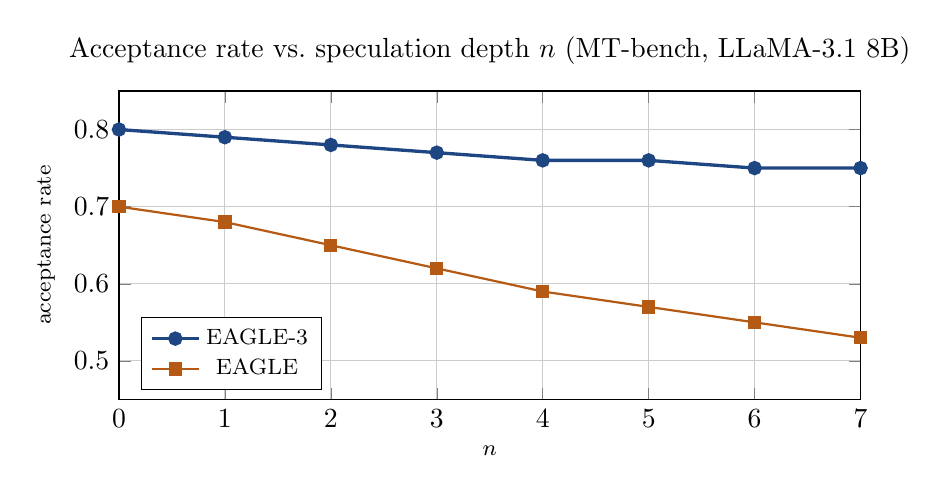
\begin{tikzpicture}
\begin{axis}[
    title={Acceptance rate vs.\ speculation depth $n$ (MT-bench, LLaMA-3.1 8B)},
    xlabel={$n$},
    ylabel={acceptance rate},
    xmin=0, xmax=7, ymin=0.45, ymax=0.85,
    grid=both,
    major grid style={black!20},
    minor grid style={black!8},
    width=11cm, height=5.5cm,
    legend pos=south west,
    tick style={font=\footnotesize},
    label style={font=\footnotesize},
    legend style={font=\footnotesize}
]
\addplot[accent, mark=*, very thick] coordinates {(0,0.80)(1,0.79)(2,0.78)(3,0.77)(4,0.76)(5,0.76)(6,0.75)(7,0.75)};
\addlegendentry{EAGLE-3}
\addplot[remarkorange, mark=square*, thick] coordinates {(0,0.70)(1,0.68)(2,0.65)(3,0.62)(4,0.59)(5,0.57)(6,0.55)(7,0.53)};
\addlegendentry{EAGLE}
\end{axis}
\end{tikzpicture}
\par\smallskip
{\small Schematic redraw of the slide's comparison; the curves are
approximate.}
\end{center}

EAGLE-3's acceptance rate remains in the $0.75$--$0.80$ band across all
depths, whereas the original EAGLE declines from $\approx 0.70$ at $n=0$
to below $0.55$ at $n=7$. In absolute terms, EAGLE-3 achieves roughly a
30--40\% speedup over EAGLE-2 depending on the task.

The ablation of design choices is instructive:

\begin{center}
\renewcommand{\arraystretch}{1.25}
\begin{tabular}{@{}lcccc@{}}
\toprule
\textbf{Configuration} & \textbf{Speedup} & \textbf{MT-bench} & \textbf{GSM8K speedup} & \textbf{GSM8K score} \\
\midrule
EAGLE-2                          & $3.16\times$ & 4.05 & $3.39\times$ & 4.24 \\
\quad $+$ remove feature loss    & $3.82\times$ & 5.37 & $3.77\times$ & 5.22 \\
\quad $+$ fused features (ours)  & $4.40\times$ & 6.13 & $4.48\times$ & 6.23 \\
\bottomrule
\end{tabular}
\end{center}

The lesson: feature-level distillation between drafter and target, which
intuitively ought to help, actually hurts; integrating features directly
(``fused features'') and training on a deeper token-level loss performs
substantially better.

%%%%%%%%%%%%%%%%%%%%%%%%%%%%%%%%%%%%%%%%%%%%%%%%%%%%%%%%%%%%%%%%%%%%%%%%
\section{Managing the KV Cache}
\label{sec:kv-and-beyond}
%%%%%%%%%%%%%%%%%%%%%%%%%%%%%%%%%%%%%%%%%%%%%%%%%%%%%%%%%%%%%%%%%%%%%%%%

The KV cache has been the recurring villain of these notes. It forces
small batches, it starves the experts, and its memory footprint scales
pitilessly with context length. An entire sub-discipline exists to tame
it.

\subsection{The Innate Flaws of Self-Attention}

Let us state the difficulties plainly. For a sequence of length $L$:

\begin{itemize}[leftmargin=1.5em, itemsep=2pt]
  \item \textbf{Per-step cost:} $\bigO(L)$ to attend to the full history.
  \item \textbf{Total cost:} $\bigO(L^2)$ to process the full sequence.
  \item \textbf{VRAM demand:} $\bigO(L)$ for the cache, per sequence, per
        batch element.
  \item \textbf{Bottleneck:} memory-bound during decoding, with poor
        scaling for long contexts.
\end{itemize}

At $L = 128\text{K}$, a vanilla KV cache forces batch sizes so small that
latency degrades unacceptably. The engineering response partitions into
several orthogonal strategies.

\subsection{Taxonomy of Optimisations}

\begin{center}
\renewcommand{\arraystretch}{1.25}
\begin{tabular}{@{}p{0.28\textwidth} p{0.32\textwidth} p{0.32\textwidth}@{}}
\toprule
\textbf{Technique} & \textbf{Definition} & \textbf{Primary benefit} \\
\midrule
Token-level pruning        & Identify and skip unimportant tokens within the attention kernel & Reduced effective $L$ \\
Cache budget allocation    & Impose fixed memory caps per layer or per head & Predictable VRAM \\
Cache merging              & Combine multiple KV pairs into summary pairs, within or across layers & Reduced cache volume \\
Quantization               & Store KV tensors at INT8 or INT4 precision & Smaller footprint \\
Offloading                 & Move cache to DRAM, SSD, or network storage & Supports longer contexts \\
Low-rank decomposition     & Approximate $W \approx UV^\top$ with $r \ll \min(n,m)$ & Fewer parameters \\
\bottomrule
\end{tabular}
\end{center}

\subsection{Exploiting Attention Sparsity}

A key empirical observation: attention maps of trained models are
overwhelmingly \emph{sparse}. For any given query, only a small fraction
of the preceding context (often around $5\%$) carries meaningful weight.
The rest of the map is essentially black.

This has a crucial consequence. The context \emph{required to generate a
particular token} is much smaller than the context \emph{available in the
cache}. If we could identify which KV pairs the current query will
actually attend to, we could pass only those to the attention
kernel---dramatically reducing the per-step work without evicting anything
from the cache.

\begin{principle}[Selection versus eviction]
Standard cache-management techniques evict tokens permanently to save
memory. An alternative is to \emph{keep} all tokens in VRAM but \emph{pass}
only a selected subset into the attention kernel at each step---made
practical at the serving-system level by page-table-style cache managers
such as PagedAttention.\footnote{W.\ Kwon et al., ``Efficient Memory
Management for Large Language Model Serving with PagedAttention'' (SOSP
2023), \arxivlink{2309.06180}.} The full cache remains available for future
queries that may need it; only the kernel load is reduced. This
``selective-passing'' or ``sparse attention'' view is the organising idea
of techniques like DeepSeek's DSA.
\end{principle}

\subsection{Low-Rank KV Compression and MLA}

A complementary angle is to compress the cache itself. Rather than storing
$K$ and $V$ at their full hidden dimension, project them through a
low-rank factor of dimension $r \ll d$. Memory is reduced by a factor of
$d/r$; at retrieval, an up-projection recovers the original. The added
compute is mild and can often be hidden behind other work. This is the
idea underlying \textbf{Multi-head Latent Attention}
(MLA)\footnote{DeepSeek-AI, ``DeepSeek-V2: A Strong, Economical, and
Efficient Mixture-of-Experts Language Model'' (2024),
\arxivlink{2405.04434}.} and related techniques---particularly
well-suited to short- and medium-context regimes.

\subsection{Dynamic Sparse Attention (DSA)}

DeepSeek-V3.2\footnote{DeepSeek-AI, ``DeepSeek-V3.2: Pushing the Frontier
of Open Large Language Models'' (2025), \arxivlink{2512.02556}.}
synthesises the two ideas: low-rank latent attention (MLA) plus a learned
top-$k$ selection over the cache. The core computation introduces a
lightweight \emph{index} that ranks cached tokens by relevance:
\begin{equation}
  I_{i,s} \;=\; \sum_{j=1}^{H} w'_{i,j}\, \operatorname{ReLU}(\mathbf{q}'_{i,j} \cdot \mathbf{k}'_j),
\end{equation}
with a KL-based training loss encouraging $\operatorname{softmax}(I_{i,s})$
to match the ground-truth attention distribution:
\begin{equation}
  \mathcal{L} \;=\; \sum_i \KL\!\left(P_{i,s} \,\big\|\, \operatorname{softmax}(I_{i,s})\right).
\end{equation}

The architecture proper uses a lightning indexer and a top-$k$ selector
atop Multi-Query Attention, with RoPE positional embeddings and
block-structured access patterns to exploit the fact that memory transfer
costs scale with block size, not element count:

\begin{center}
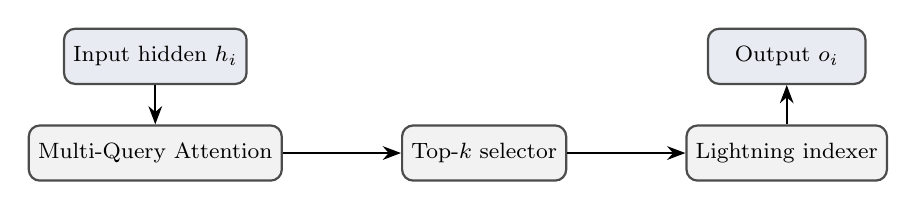
\begin{tikzpicture}[
  every node/.style={font=\footnotesize},
  box/.style={rectangle, rounded corners, draw=black!70, thick, minimum height=0.7cm,
              minimum width=2cm, fill=gray!10, align=center},
  acc/.style={rectangle, rounded corners, draw=black!70, thick, minimum height=0.7cm,
              minimum width=2cm, fill=accent!10, align=center},
  arrow/.style={-Stealth, thick}
]
  \node[acc] (in) {Input hidden $h_i$};
  \node[box, below=0.5cm of in] (mqa) {Multi-Query Attention};
  \node[box, right=1.5cm of mqa] (topk) {Top-$k$ selector};
  \node[box, right=1.5cm of topk] (indexer) {Lightning indexer};
  \node[acc, above=0.5cm of indexer] (out) {Output $o_i$};

  \draw[arrow] (in) -- (mqa);
  \draw[arrow] (mqa) -- (topk);
  \draw[arrow] (topk) -- (indexer);
  \draw[arrow] (indexer) -- (out);
\end{tikzpicture}
\end{center}

The block-structured access is a hardware-aware optimisation: since
retrieving one element from VRAM costs roughly as much as retrieving a
block of 128 contiguous elements, accessing data in blocks is essentially
free per element.

\subsection{System-Level Extensions}

Above the kernel level sit broader strategies: \emph{prefix sharing}
(reuse context processing across requests that begin alike), \emph{load
balancing} across heterogeneous clusters, \emph{cascades} of models, and
agent-specific optimisations. Once a cache exceeds on-chip memory, an
offloading hierarchy---HBM $\to$ DRAM $\to$ SSD $\to$ network
storage---extends effective context at proportional latency cost.

%%%%%%%%%%%%%%%%%%%%%%%%%%%%%%%%%%%%%%%%%%%%%%%%%%%%%%%%%%%%%%%%%%%%%%%%
\section{Linear Attention and State-Space Models}
\label{sec:linear}
%%%%%%%%%%%%%%%%%%%%%%%%%%%%%%%%%%%%%%%%%%%%%%%%%%%%%%%%%%%%%%%%%%%%%%%%

The most ambitious response to the quadratic cost of self-attention is to
replace it outright. Linear-attention architectures---Mamba\footnote{A.\
Gu, T.\ Dao, ``Mamba: Linear-Time Sequence Modeling with Selective State
Spaces'' (2023), \arxivlink{2312.00752}.}, GatedDeltaNet\footnote{S.\
Yang, J.\ Kautz, A.\ Hatamizadeh, ``Gated Delta Networks: Improving Mamba2
with Delta Rule'' (2024), \arxivlink{2412.06464}.}, and the
linear-attention blocks of Qwen3-Next---maintain a fixed-size recurrent
state rather than a growing cache, and therefore process a token in
$\bigO(1)$ rather than $\bigO(L)$.

\subsection{The GatedDeltaNet Recurrence}

A representative recurrence governs how the state $S_t$ evolves as the
model reads token $t$:
\begin{equation}
  S_t \;=\; S_{t-1}\bigl(\alpha_t (I - \beta_t k_t k_t^\top)\bigr) + \beta_t v_t k_t^\top,
  \label{eq:gdn}
\end{equation}
where $\alpha_t, \beta_t \in [0,1]$ are gating scalars derived from the
current input and $k_t, v_t$ are key and value vectors. The first term
\emph{decays} the existing state along the direction $k_t$ (a soft
forget); the second \emph{writes} the new value into that direction. The
update is a rank-one correction of the state matrix---a differentiable
generalisation of a hash-table write.

\subsection{Hybrid Architectures}

In practice, pure linear-attention stacks underperform on tasks requiring
exact lookup (copying, factual recall); they compress history too
aggressively. Modern deployments therefore \emph{interleave}: three
GatedDeltaNet blocks followed by one standard full-attention block,
repeated. The linear blocks carry the long-range state efficiently; the
occasional full-attention block provides exact retrieval.

\begin{center}
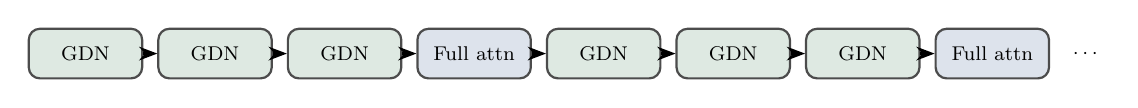
\begin{tikzpicture}[
  block/.style={rectangle, rounded corners, draw=black!70, thick, minimum width=1.6cm,
                minimum height=0.7cm, font=\footnotesize, align=center},
  gdn/.style={block, fill=defgreen!15},
  full/.style={block, fill=accent!15},
  arrow/.style={-Stealth, thick},
  scale=0.9, transform shape
]
  \node[gdn] (g1) {GDN};
  \node[gdn, right=0.2cm of g1] (g2) {GDN};
  \node[gdn, right=0.2cm of g2] (g3) {GDN};
  \node[full, right=0.2cm of g3] (f1) {Full attn};
  \node[gdn, right=0.2cm of f1] (g4) {GDN};
  \node[gdn, right=0.2cm of g4] (g5) {GDN};
  \node[gdn, right=0.2cm of g5] (g6) {GDN};
  \node[full, right=0.2cm of g6] (f2) {Full attn};
  \node[right=0.2cm of f2, font=\footnotesize] {$\cdots$};

  \draw[arrow] (g1) -- (g2);
  \draw[arrow] (g2) -- (g3);
  \draw[arrow] (g3) -- (f1);
  \draw[arrow] (f1) -- (g4);
  \draw[arrow] (g4) -- (g5);
  \draw[arrow] (g5) -- (g6);
  \draw[arrow] (g6) -- (f2);
\end{tikzpicture}
\end{center}

\subsection{Throughput Profile}

The payoff is most visible at long contexts:

\begin{center}
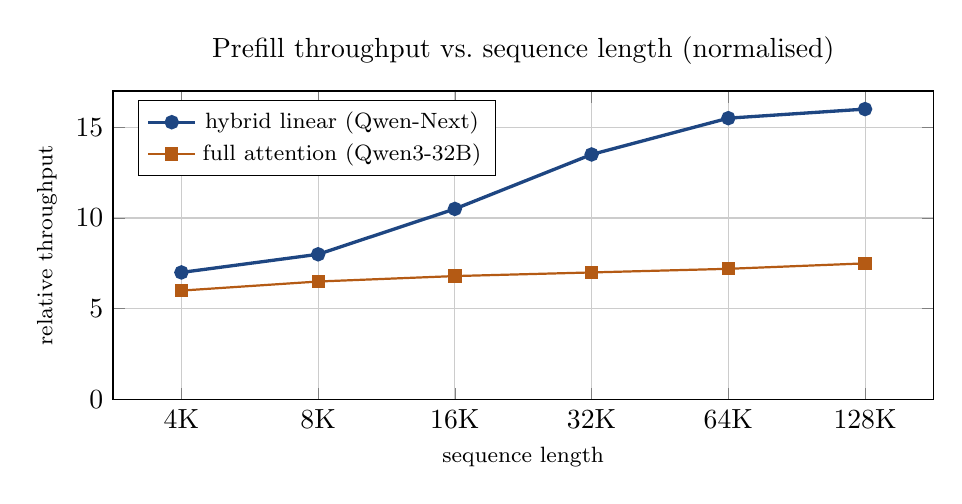
\begin{tikzpicture}
\begin{axis}[
    title={Prefill throughput vs.\ sequence length (normalised)},
    xlabel={sequence length},
    ylabel={relative throughput},
    xmode=log,
    log basis x={2},
    ymin=0, ymax=17,
    xtick={4000, 8000, 16000, 32000, 64000, 128000},
    xticklabels={4K, 8K, 16K, 32K, 64K, 128K},
    grid=both,
    major grid style={black!20},
    minor grid style={black!8},
    width=12cm, height=5.5cm,
    legend pos=north west,
    tick style={font=\footnotesize},
    label style={font=\footnotesize},
    legend style={font=\footnotesize}
]
\addplot[accent, mark=*, very thick] coordinates {(4000,7)(8000,8)(16000,10.5)(32000,13.5)(64000,15.5)(128000,16)};
\addlegendentry{hybrid linear (Qwen-Next)}
\addplot[remarkorange, mark=square*, thick] coordinates {(4000,6)(8000,6.5)(16000,6.8)(32000,7)(64000,7.2)(128000,7.5)};
\addlegendentry{full attention (Qwen3-32B)}
\end{axis}
\end{tikzpicture}
\par\smallskip
{\small Schematic redraw of the slide's throughput comparison; the values
are approximate.}
\end{center}

\subsection{Implementation Realities}

The theory of linear attention is clean; the implementation is not.
Training requires a \emph{chunkwise-parallel} reformulation of
Equation~\eqref{eq:gdn}---the naive recurrence is sequential and cannot
use Tensor cores, so the sequence is split into chunks, each chunk's
intra-chunk contribution is computed as a (parallelisable) matrix product,
and only the small inter-chunk state is carried recurrently. Current open
kernels (Triton-based, e.g.\ the Flash Linear Attention library) carry
significant CPU launch overhead relative to their tiny per-step FLOP
count, use non-standard convolutional primitives for the short-context
gating, and require careful management of fixed-state buffers and
cache-reuse semantics for long-context inference. These are
first-generation tools, improving rapidly but not yet at the engineering
maturity of FlashAttention.

%%%%%%%%%%%%%%%%%%%%%%%%%%%%%%%%%%%%%%%%%%%%%%%%%%%%%%%%%%%%%%%%%%%%%%%%
\section{Knowledge Distillation}
\label{sec:kd}
%%%%%%%%%%%%%%%%%%%%%%%%%%%%%%%%%%%%%%%%%%%%%%%%%%%%%%%%%%%%%%%%%%%%%%%%

A final class of techniques addresses not the inference path but the model
itself. In \emph{knowledge distillation} (KD)\footnote{G.\ Hinton,
O.\ Vinyals, J.\ Dean, ``Distilling the Knowledge in a Neural Network''
(2015), \arxivlink{1503.02531}.} we train a small \emph{student} model
$q_\theta$ to imitate a large \emph{teacher} model $p$. The deployed
artefact is the student; the teacher, once consulted, can be discarded.

\begin{definition}[Knowledge distillation objective]
Let $p(y \mid x)$ be the teacher's conditional distribution and
$q_\theta(y\mid x)$ the student's. Knowledge distillation minimises
\[
  \mathcal{L}\bigl(p(y\mid x),\, q_\theta(y\mid x)\bigr) \;\longrightarrow\; \min_\theta,
\]
where $\mathcal{L}$ is an appropriate divergence between distributions.
\end{definition}

\subsection{Hard-Label Distillation}

The simplest realisation samples a large corpus of generations from the
teacher and trains the student on them with the ordinary cross-entropy
loss, exactly as if the generations were ground truth:
\[
  \{x^{(n)}, y^{(n)}\}_{n=1}^N, \qquad y^{(n)} \sim p(\cdot \mid x^{(n)}).
\]
This is robust and widely used, but \emph{data-hungry}: one routinely
needs millions of generation--target pairs for a strong student. It is also
wasteful of information: the teacher's full predictive distribution is
collapsed to a single sampled token.

A richer hard-label variant uses a reward model (RM) to rerank teacher
samples: the SFT model generates $n$ candidates, the RM selects the best,
and the student is trained on the selected. This is the foundation of
reinforcement-learning-from-comparison-data pipelines and exploits the
teacher's generation capability more efficiently.

\subsection{Soft-Label Distillation}

If the teacher is available during training---even as a fixed
reference---we can match its entire output distribution. The natural loss
is the Kullback--Leibler divergence,
\begin{equation}
  \KL\bigl(p(y\mid x) \,\|\, q_\theta(y\mid x)\bigr) \;=\; \E_{p(y\mid x)}\!\left[\log \frac{p(y\mid x)}{q_\theta(y\mid x)}\right],
  \label{eq:kl}
\end{equation}
evaluated and averaged over tokens and examples. This captures not only
which token the teacher would choose but \emph{how confident} it is and
\emph{what the plausible alternatives are}. For each input, the student
learns the shape of the teacher's uncertainty.

\subsection{The Mode-Matching Problem}

Matching a distribution with another is not always well-posed. Suppose the
teacher is multimodal---its distribution over outputs has several peaks,
corresponding to stylistically distinct but equally valid completions. If
the student's architecture is effectively unimodal (a single strong peak),
minimising the \emph{forward} KL $\KL(p \,\|\, q_\theta)$ will force the
student to \emph{cover} the support of the teacher, producing a blurry
average that matches no mode cleanly.

The alternative is the \emph{reverse} KL,
\begin{equation}
  \KL\bigl(q_\theta \,\|\, p\bigr) \;=\; \E_{q_\theta}\!\left[\log \frac{q_\theta(y)}{p(y)}\right],
\end{equation}
which is mode-\emph{seeking}: the student concentrates on a single
well-supported mode, accepting that it cannot model the others. Whether
forward or reverse KL is preferable depends on the downstream task---reverse
KL is standard in reinforcement-learning contexts such as PPO, where
committing to one good action is preferable to averaging many.

\subsection{Scaling: The Storage Problem}

Soft-label KD faces a hard engineering obstacle. A modern vocabulary has
$V \sim 128\text{K}$ tokens; storing the full teacher distribution for
every token of every training example demands storage approaching the
petabyte scale. A ``dirty hack'' is to recompute teacher logits in
parallel during training, avoiding the storage entirely, but this requires
the teacher to be hosted alongside the student---doubling the compute
requirement.


The \emph{SLIM} (Sparse-Label Info-Maximisation) approach exploits a
characteristic property of trained LLMs: the teacher's distribution is
extremely concentrated. Typically $99\%$ of the probability mass sits on
the top five tokens. Storing only those top-$k$ entries---values and
indices---captures nearly all of the information at a tiny fraction of the
cost.

In practice, keeping the top $5\%$ of logits per token suffices to match
full-distribution distillation quality while reducing storage by orders of
magnitude.

A clean synthesis: during training, let the student generate tokens; at
each generated token, check whether it falls within the teacher's top-$k$.
Encourage generations that land in the top-$k$; penalise those that do
not. This sidesteps the need to backpropagate through the sampling
operation---a hard and expensive trick---while keeping the student's
trajectories aligned with the teacher's preferences. Speculative Knowledge Distillation(SKD) composes
naturally with SLIM's sparse logit storage, giving a practical, scalable
soft-label pipeline.

%%%%%%%%%%%%%%%%%%%%%%%%%%%%%%%%%%%%%%%%%%%%%%%%%%%%%%%%%%%%%%%%%%%%%%%%
\section{Synthesis: A Checklist of Principles}
\label{sec:close}
%%%%%%%%%%%%%%%%%%%%%%%%%%%%%%%%%%%%%%%%%%%%%%%%%%%%%%%%%%%%%%%%%%%%%%%%

The techniques surveyed above span four orders of magnitude in
scope---from single-bit arithmetic decisions to cluster-level
scheduling---but they reduce to a small number of recurring manoeuvres.
Stated explicitly:

\begin{enumerate}[leftmargin=1.8em, itemsep=2pt]
  \item \textbf{Identify the regime.} Every kernel is either compute-bound
        or memory-bound (Section~\ref{sec:hardware}); the correct
        optimisation differs categorically between the two, and prefill
        and decode are rarely in the same regime
        (Section~\ref{sec:two-phases}).
  \item \textbf{Migrate difficulty, do not destroy it.} SmoothQuant
        (Eq.~\eqref{eq:smooth-invariance}) and SpinQuant both exploit an
        exact invariance of the computation to relocate numerical
        difficulty from a component that cannot absorb it to one that can;
        clipping or destroying information outright
        (Section~\ref{sec:smoothquant}) is rarely an option.
  \item \textbf{Trade memory for batch size, and batch size for
        throughput.} GQA, FP8 KV-cache compression, MLA, and cache
        offloading are all, mechanically, the same lever applied at
        different points of Eq.~\eqref{eq:kv-size} and
        Eq.~\eqref{eq:vram-budget}.
  \item \textbf{Exploit sparsity in the workload, not only in the
        weights.} Most tokens are easy (speculative decoding), most
        attention weight is concentrated on a few keys (DSA,
        Section~\ref{sec:kv-and-beyond}), and most teacher probability mass
        sits on a handful of tokens (SLIM, Section~\ref{sec:kd}).
  \item \textbf{Never report a speedup without its overhead.}
        Quantize/dequantize costs, drafter forward passes, and rotation
        kernels all eat into the headline number; the only honest
        benchmark is end-to-end.
\end{enumerate}

A final caution on durability: techniques tied to a specific hardware
generation age quickly. Hadamard rotations were essential for MXFP4 and
largely redundant for NVFP4 once block-level scaling matured
(Section~\ref{sec:fp4})---not because the idea was wrong, but because the
hardware absorbed it. The transferable asset is fluency with the five
principles above, not attachment to any single implementation of them.

%%%%%%%%%%%%%%%%%%%%%%%%%%%%%%%%%%%%%%%%%%%%%%%%%%%%%%%%%%%%%%%%%%%%%%%%
\section{References}
\label{sec:refs}
%%%%%%%%%%%%%%%%%%%%%%%%%%%%%%%%%%%%%%%%%%%%%%%%%%%%%%%%%%%%%%%%%%%%%%%%

\begin{enumerate}[leftmargin=1.8em, itemsep=3pt]
\item E.\ Frantar, S.\ Ashkboos, T.\ Hoefler, D.\ Alistarh. \textit{GPTQ: Accurate Post-Training Quantization for Generative Pre-trained Transformers.} 2022. \arxivlink{2210.17323}.
\item G.\ Xiao, J.\ Lin, M.\ Seznec, H.\ Wu, J.\ Demouth, S.\ Han. \textit{SmoothQuant: Accurate and Efficient Post-Training Quantization for Large Language Models.} 2022. \arxivlink{2211.10438}.
\item P.\ Micikevicius et al. \textit{FP8 Formats for Deep Learning.} 2022. \arxivlink{2209.05433}.
\item Z.\ Liu et al. \textit{SpinQuant: LLM Quantization with Learned Rotations.} 2024 (ICLR 2025). \arxivlink{2405.16406}.
\item Open Compute Project. \textit{OCP Microscaling Formats (MX) Specification v1.0.} 2023. \href{https://www.opencompute.org/documents/ocp-microscaling-formats-mx-v1-0-spec-final-pdf}{opencompute.org}.
\item NVIDIA. \textit{Introducing NVFP4 for Efficient and Accurate Low-Precision Inference.} 2024. \href{https://developer.nvidia.com/blog/introducing-nvfp4-for-efficient-and-accurate-low-precision-inference/}{developer.nvidia.com}.
\item N.\ Shazeer. \textit{Fast Transformer Decoding: One Write-Head is All You Need.} 2019. \arxivlink{1911.02150}.
\item J.\ Ainslie, J.\ Lee-Thorp, M.\ de Jong, Y.\ Zemlyanskiy, F.\ Lebr\'on, S.\ Sanghai. \textit{GQA: Training Generalized Multi-Query Transformer Models from Multi-Head Checkpoints.} 2023. \arxivlink{2305.13245}.
\item W.\ Fedus, B.\ Zoph, N.\ Shazeer. \textit{Switch Transformers: Scaling to Trillion Parameter Models with Simple and Efficient Sparsity.} 2021. \arxivlink{2101.03961}.
\item T.\ Dao, D.\ Fu, S.\ Ermon, A.\ Rudra, C.\ R\'e. \textit{FlashAttention: Fast and Memory-Efficient Exact Attention with IO-Awareness.} NeurIPS 2022.
\item T.\ Dao. \textit{FlashAttention-2: Faster Attention with Better Parallelism and Work Partitioning.} 2023. \arxivlink{2307.08691}.
\item J.\ Shah, G.\ Bikshandi, Y.\ Zhang, V.\ Thakkar, P.\ Ramani, T.\ Dao. \textit{FlashAttention-3: Fast and Accurate Attention with Asynchrony and Low-precision.} 2024. \arxivlink{2407.08608}.
\item Y.\ Leviathan, M.\ Kalman, Y.\ Matias. \textit{Fast Inference from Transformers via Speculative Decoding.} ICML 2023. \arxivlink{2211.17192}.
\item C.\ Chen, S.\ Borgeaud, G.\ Irving, J.-B.\ Lespiau, L.\ Sifre, J.\ Jumper. \textit{Accelerating Large Language Model Decoding with Speculative Sampling.} 2023. \arxivlink{2302.01318}.
\item Y.\ Li, F.\ Wei, C.\ Zhang, H.\ Zhang. \textit{EAGLE: Speculative Sampling Requires Rethinking Feature Uncertainty.} 2024. \arxivlink{2401.15077}.
\item Y.\ Li, F.\ Wei, C.\ Zhang, H.\ Zhang. \textit{EAGLE-2: Faster Inference of Language Models with Dynamic Draft Trees.} 2024. \arxivlink{2406.16858}.
\item Y.\ Li et al. \textit{EAGLE-3: Scaling up Inference Acceleration of Large Language Models via Training-Time Test.} 2025. \arxivlink{2503.01840}.
\item W.\ Kwon et al. \textit{Efficient Memory Management for Large Language Model Serving with PagedAttention.} SOSP 2023. \arxivlink{2309.06180}.
\item DeepSeek-AI. \textit{DeepSeek-V2: A Strong, Economical, and Efficient Mixture-of-Experts Language Model.} 2024. \arxivlink{2405.04434}.
\item DeepSeek-AI. \textit{DeepSeek-V3.2: Pushing the Frontier of Open Large Language Models.} 2025. \arxivlink{2512.02556}.
\item A.\ Gu, T.\ Dao. \textit{Mamba: Linear-Time Sequence Modeling with Selective State Spaces.} 2023. \arxivlink{2312.00752}.
\item S.\ Yang, J.\ Kautz, A.\ Hatamizadeh. \textit{Gated Delta Networks: Improving Mamba2 with Delta Rule.} 2024. \arxivlink{2412.06464}.
\item G.\ Hinton, O.\ Vinyals, J.\ Dean. \textit{Distilling the Knowledge in a Neural Network.} 2015. \arxivlink{1503.02531}.
\end{enumerate}

\end{document}